% concatenated from EAgroups_20260320.tex


\documentclass{amsart}
%\usepackage[left=2.50cm, right=2.50cm, top=2.50cm, bottom=2.50cm]{geometry}

%\usepackage{geometry}
%\usepackage{helvet}
\usepackage{amsthm,amsmath, amsfonts, amssymb, comment}
\newtheorem{theorem}{Theorem}[section]
\newtheorem{lemma}[theorem]{Lemma}
\newtheorem{proposition}[theorem]{Proposition}
\newtheorem{corollary}[theorem]{Corollary}
\newtheorem{question}[theorem]{Question}
\newtheorem*{conjecture}{Conjecture}
\theoremstyle{definition}
\newtheorem{definition}{Definition}[section]
\newtheorem*{programme}{Program}
\theoremstyle{remark}
\newtheorem*{remark}{Remark}
\usepackage{mathrsfs}
\usepackage[english]{babel}
\usepackage{graphicx}   
\usepackage{tikz}
\usepackage{subcaption}
\usepackage{url}        
\usepackage{bm}         
\usepackage{multirow}
\usepackage{booktabs}
\usepackage{algorithm}
\usepackage{algorithmic}
\usepackage{enumerate}
\renewcommand{\algorithmicrequire}{ \textbf{Input:}}
\renewcommand{\algorithmicensure}{ \textbf{Initialize:}}
\renewcommand{\algorithmicreturn}{ \textbf{Output:}}
%\usepackage{fancyhdr} 
%\pagestyle{fancy}
%\lhead{}
%\chead{}
%\lfoot{}
%\cfoot{}
%\rfoot{}
\usepackage[colorlinks, linkcolor=black]{hyperref} 
\providecommand*{\lemmaautorefname}{Lemma}
\providecommand*{\claimautorefname}{Claim}
\providecommand*{\remarkautorefname{Remark}}
\hypersetup{colorlinks, bookmarks, unicode} 
\usepackage{multicol}
\usepackage[noadjust]{cite}
\usepackage{indentfirst}




\begin{document}

\title[Extremely Amenable Automorphism Groups]{Extremely Amenable Automorphism Groups of Countable Structures}

\author{Mahmood Etedadialiabadi}
\address{1979 Milky Way, Verona, WI 53593, U.S.A.}
\email{mahmood.etedadi@gmail.com}

\author{Su Gao}
\address{School of Mathematical Sciences and LPMC, Nankai University, Tianjin 300071, P.R. China}
\email{sgao@nankai.edu.cn}
\thanks{S. Gao and the F. Li acknowledge the partial support of their research by the National Natural Science Foundation of China (NSFC) grants 12271263 and 12250710128. R. Li acknowledges the partial support of his research by the NSFC grant 124B2001. S. Gao, F. Li and R. Li attended the Tianyuan Workshop on Computability Theory and Descriptive Set Theory in June 2025 when a part of this research was conducted, and we acknowledge the support by the Tianyuan Mathematics Research Center.}
\subjclass[2020]{22F05, 54H05}
\author{Feng Li}
\address{School of Mathematical Sciences and LPMC, Nankai University, Tianjin 300071, P.R. China}
\email{fengli@mail.nankai.edu.cn}

\author{Ruiwen Li}
\address{School of Mathematical Sciences and LPMC, Nankai University, Tianjin 300071, P.R. China}
\email{rwli@mail.nankai.edu.cn}

%\date{\today}

    
\begin{abstract}  In this paper we address the question: How many pairwise non-isomorphic extremely amenable groups are there which are separable metrizable or even Polish? We show that there are continuum many such groups. In fact we construct continuum many pairwise non-isomorphic extremely amenable groups as automorphism groups of countable structures. We also consider this classification problem from the point of view of descriptive set theory by showing that the class of all extremely amenable closed subgroups of $S_\infty$ is Borel and their isomorphism relation is more complex than any isomorphism relation of countable structures in the Borel reducibility hierarchy. 
\end{abstract}

\maketitle
%\tableofcontents
\section{Introduction}    

A topological group $G$ is extremely amenable if for every continuous action of $G$ on a compact Hausdorff space $X$, there is a fixed point $x\in X$, i.e., for all $g\in G$, $g\cdot x=x$. This is a remarkable property for a topological group to have. In fact, Veech \cite{Veech} proved that no locally compact topological groups can be extremely amenable. This explained why extremely amenable groups were not present in the early development of topological group theory, for instance in the study of Hilbert's fifth problem. 

Ever since Mitchell \cite{Mitchell} asked in 1970 about the existence of non-trivial extremely amenable topological groups, many examples of such groups have been discovered. At first, these groups were thought to be pathological since they had to be obtained via intricate constructions. However, as time goes by, more familiar groups have been shown to be extremely amenable. The extremely amenable groups we now know of can be loosely sorted into three classes as follows.

The first examples of extremely amenable groups were given by Herer--Christensen \cite{HC}. 
They constructed such groups which are abelian Polish groups of the form $L_0(\mu, \mathbb{R})$, which is the additive group of all $\mathbb{R}$-valued $\mu$-measurable functions, where $\mu$ is a pathological submeasure. Later, other examples of the more general form $L_0(\mu, G)$, where $G$ is a topological group, were shown to be extremely amenable. Among them, Furstenberg--Weiss (in unpublished work) and independently Glasner \cite{Glasner} showed that the group of measurable maps from the unit interval $\mathbb{I}$ with the Lebesgue measure $\lambda$ to the unit circle $\mathbb{T}$ is extremely amenable.  Farah--Solecki \cite{FS2008} generalized it by showing that $L_0(\mu, G)$ is extremely amenable when $G$ is a compact solvable topological group and $\mu$ is a so-called diffused submeasure. Sabok \cite{Marcin} generalized further to arbitrary solvable topological groups $G$ and diffused submeaures $\mu$. 
% In Sabok's paper, he incorrectly stated that Pestov showed the extreme amenability for diffused submeasure $\mu$ and amenable $G$. Pestov never stated or proved this claim.

In a different thread of research, many operator groups were also shown to be extremely amenable. Famously, Gromov--Milman \cite{GM} showed that the unitary group $U(H)$ of the infinite dimensional separable Hilbert space $H$ is extremely amenable. Pestov proved the extreme amenability for the group $\mbox{Homeo}_+(\mathbb{I})$ of all order-preserving homeomorphisms of the unit interval (\cite{Pestov98}) and for the group $\mbox{\rm Iso}(\mathbb{U})$ of all isometries of the universal Urysohn metric space $\mathbb{U}$ (\cite{Pestov02}).  Giordano--Pestov \cite{GP} showed the extreme amenability for $\mbox{\rm Aut}(\mathbb{I},\lambda)$, the group of all measure-preserving automorphisms of the Lebesgue space.

A third class of topological groups known to be extremely amenable in the literature comes from automorphism groups of countable structures. Pestov \cite{Pestov98} gave the first example of such a group, which is ${\rm Aut}(\mathbb{Q}, <)$, the automorphism group of a countable dense linear order without endpoints. Motivated by the idea in \cite{Pestov98}, Kechris--Pestov--Todorcevic \cite{KPT} gave a complete characterization of when the automorphism group of a countable structure is extemely amenable, which is now called the KPT correspondence. The KPT correspondence connects the extreme amenability to the so-called structural Ramsey property of Fra\"iss\'e classes and gives a number of examples of extremely amenable groups.  Through the work of Ne\v{s}et\v{r}il--R\"{o}dl \cite{NR77} \cite{NR83} and Ne\v{s}et\v{r}il \cite{Nes07} on Ramsey classes, we now have extremely amenable groups of the form $\mbox{\rm Aut}(M)$, where $M$ is the Fra\"{\i}ss\'{e} limit of a Fra\"{\i}ss\'{e} class of countable structures. Such structures include ordered graphs, ordered $K_n$-free graphs, ordered $\mathbb{Q}$-metric spaces, and ordered $\mathbb{N}$-metric spaces, etc. The KPT correspondence has also been generalized to the context of continuous logic by Melleray--Tsankov \cite{MT}.

Despite the diversity of these examples, not much was known about the number of distinct isomorphism types of extremely amenable groups. Among the above examples, only finitely many pairwise non-isomorphic extremely amenable groups can be identified. This motivates us to study the following question: How many pairwise non-isomorphic extremely amenable groups are there? 

The only result that explicitly addressed this question in the literature is a theorem of Pestov in \cite{Pestov98}, which states that for each infinite cardinal $\kappa$, there is an extremely amenable topological group of weight $\kappa$. Since the weight is an isomorphism invariant, we obtain many pairwise non-isomorphic extremely amenable groups. However, we would like to study this question in the context of more familiar groups, in particular separable metrizable groups and Polish groups. The theorem of Pestov gives only one such example. 

Our main results of the paper confirm that there are continuum many non-isomorphic extremely amenable groups which are either Polish or separable metrizable. Our study focuses on the third class of examples in the above review. 

The first main result of this paper confirms that there are continuum many pairwise non-isomorphic extremely amenable groups that are separable and metrizable. For each countable distance value set $\Delta$ (to be defined in Section~\ref{sec:2}), we consider the $\Delta$-metric Urysohn space $\mathbb{U}_\Delta$. The group $\mbox{\rm Iso}(\mathbb{U}_\Delta)$ of all isometries of $\mathbb{U}_\Delta$, equipped with the topology of pointwise convergence in metric, is a separable metrizable group. We show the following theorems.

\begin{theorem}\label{thm:main1} Let $\Delta$ be a countable distance value set. Then the following hold:
\begin{enumerate}
\item[\rm (1)] $\mbox{\rm Iso}(\mathbb{U}_\Delta)$ is extremely amenable if and only if $\inf\Delta=0$.
\item[\rm (2)] $\mbox{\rm Iso}(\mathbb{U}_\Delta)$ is Polish if and only if $\inf\Delta>0$.
\item[\rm (3)] If $\inf\Delta=0$, then $\mbox{\rm Iso}(\mathbb{U}_\Delta)$ is isomorphic to a dense subgroup of either $\mbox{\rm Iso}(\mathbb{U})$ or $\mbox{\rm Iso}(\mathbb{U}_1)$, where $\mathbb{U}_1$ is the Urysohn sphere, i.e., the unit sphere of $\mathbb{U}$.
\end{enumerate}
\end{theorem}

\begin{theorem}\label{thm:main2} Let $\Delta$ and $\Lambda$ be countable distance value sets. Then the following are equivalent:
\begin{enumerate}
\item[\rm (i)] $\mbox{\rm Iso}(\mathbb{U}_\Delta)$ and $\mbox{\rm Iso}(\mathbb{U}_\Lambda)$ are isomorphic as topological groups.
\item[\rm (ii)] $\mbox{\rm Iso}(\mathbb{U}_\Delta)$ and $\mbox{\rm Iso}(\mathbb{U}_\Lambda)$ are isomorphic as abstract groups.
\item[\rm (iii)] $\Delta$ and $\Lambda$ are equivalent.
\end{enumerate}
\end{theorem}


\begin{theorem}\label{thm:main3} There are continnum many pairwise inequivalent countable distance value sets $\Delta$ that are dense in $(0,+\infty)$. Consequently, there are continuum many pairwise non-isomorphic extremely amenable groups $\mbox{\rm Iso}(\mathbb{U}_\Delta)$ that are separable metrizable.
\end{theorem}

In fact, all groups in this class are dense in $\mbox{\rm Iso}(\mathbb{U})$; in particular, none of them are Polish.

We then study the case of Polish groups. Here we consider the Fra\"{\i}ss\'{e} class of all finite ordered $\Delta$-metric spaces and its Fra\"{\i}ss\'{e} limit $\mathbb{U}^{<}_{\Delta}$. Regarding $\mathbb{U}^{<}_{\Delta}$ as a countable structure, the automorphism group $\mbox{\rm Aut}(\mathbb{U}^{<}_{\Delta})$, equipped with the topology of pointwise convergence where the underlying space has the discrete topology, is a Polish group. In fact, it is isomorphic to a closed subgroup of $S_\infty$, the infinite permutation group. We use the following consequence of a theorem of Ne\v{s}et\v{r}il \cite{Nes07} (for a more explicit restatement of Ne\v{s}et\v{r}il's theorem, see Theorem 13 of Nguyen Van Th\'e \cite{NVTMAMS}).

\begin{theorem}\label{thm:main4} Let $\Delta$ be a countable distance value set. Then $\mbox{\rm Aut}(\mathbb{U}^{<}_{\Delta})$ is extremely amenable.
\end{theorem}

We show the following theorems.

\begin{theorem}\label{thm:main5} Let $\Delta$ and $\Lambda$ be countable distance value sets. Then the following are equivalent:
\begin{enumerate}
\item[\rm (i)] $\mbox{\rm Aut}(\mathbb{U}^{<}_{\Delta})$ and $\mbox{\rm Aut}(\mathbb{U}^{<}_{\Lambda})$ are isomorphic as topological groups.
\item[\rm (ii)] $\Delta$ and $\Lambda$ are equivalent.
\end{enumerate}
\end{theorem}

\begin{corollary}\label{thm:main6} There are continnum many pairwise non-isomorphic extremely amenable Polish groups of the form $\mbox{\rm Aut}(\mathbb{U}^{<}_{\Delta})$.
\end{corollary}

The proofs of Theorems~\ref{thm:main2} and \ref{thm:main5} follow the outline of the proof of a similar theorem in \cite{EGLMM}.

Our study of the isomorphism types of these extremely amenable groups goes much beyond counting the number of them. Another major effort we put in this paper is to study the isomorphism relation among these extremely amenable groups from the point of view of descriptive set theory. (For an overview of the descriptive set theory of equivalence relations, see Section~\ref{sec:2}). In view of Theorems~\ref{thm:main2} and \ref{thm:main5}, this is done by studying the complexity of the equivalence relation between countable distance value sets in the Borel reducibility hierarchy. We obtain the following penetrating results.

\begin{theorem}\label{thm:main8}{\ }
\begin{enumerate}
\item[\rm (1)] The equivalence between countable distance value sets $\Delta$ with $\inf\Delta>0$ and $\sup\Delta<\infty$ is Borel bireducible with the universal $S_\infty$-orbit equivalence relation.
\item[\rm (2)] The equivalence between countable distance value sets $\Delta$ with $\inf\Delta>0$ and $\sup\Delta=\infty$ is Borel bireducible with the equivalence relation $=^+$.
\item[\rm (3)] The equivalence between countable distance value sets $\Delta$ with $\inf\Delta=0$ is strictly in between $=^+$ and $=^{++}$ in the Borel reducibility hierarchy.
\end{enumerate}
\end{theorem}

These results significantly strengthen Theorem~\ref{thm:main3} and Corollary~\ref{thm:main6}. Theorem~\ref{thm:main8} (3) is motivated by and related to the recent work of Calderoni--Marker--Motto Ros--Shani \cite{CMMRS}. 

Finally, inspired by a research program initiated by Kechris--Nies--Tent \cite{KNT}, we show that the class of extremely amenable closed subgroups of $S_\infty$ is a Borel class (this was also independently proved by Iwanow--Majcher-Iwanow (unpublished); see \cite[Section 3]{Nies}), which implies that the isomorphism relation among these groups is an analytic equivalence relation. Regarding its complexity in the Borel reducibility hierarchy, our results yield the following.

\begin{theorem}\label{thm:main7}  The isomorphism relation among extremely amenable Polish groups that are isomorphic to closed subgroups of $S_\infty$ is more complex than the universal $S_\infty$-orbit equivalence relation. In particular, it is analytic and non-Borel.
\end{theorem}



The rest of the paper is organized as follows. In Section~\ref{sec:2} we define the basic concepts and notions and give a review of the results we need to cite in this paper. In particular, we review the descriptive set theory of equivalence relations. In Section~\ref{sec:3} we prove Theorems~\ref{thm:main1} and \ref{thm:main4}. In Section~\ref{sec:5} we prove Theorems~\ref{thm:main2} and \ref{thm:main5}. In Section~\ref{sec:CDVS} we prove Theorem~\ref{thm:main8}. Finally, in Section~\ref{sec:6} we prove that the class of extremely amenable closed subgroups of $S_\infty$ is Borel, derive Theorem~\ref{thm:main7}, and state some questions left open by this paper.

{\it Acknowledgment.} We thank Filippo Calderoni, Wei Dai, Aleksander Iwanow, Andre Nies, Marcin Sabok, Assaf Shani, Simon Thomas, and V\'{\i}ctor Hugo Ya\~{n}ez for their inspiring comments on an earlier version of the paper. 






\section{Preliminaries\label{sec:2}}
In this section we review some of the basic concepts and notation we will use in the rest of the paper.

\subsection{Topological dynamics} Our standard reference for topological dynamics is \cite{AusBook}.

Our topological spaces and topological groups are all Hausdorff. 
Let $G$ be a topological group and let $X$ be a compact Hausdorff space. Let $a\colon G\times X\to X$ be a continuous action of $G$ on $X$. For $g\in G$ and $x\in X$, we also write $g\cdot x$ for $a(g,x)$. We say that $X$ is a {\em $G$-flow}. For $x\in X$, the {\em orbit} of $x$, denoted $[x]_G$, is the set $\{g\cdot x\colon g\in G\}$. We say that the $G$-flow $X$ is {\em minimal} if for every $x\in X$, $[x]_G$ is dense in $X$. 

Suppose $G$ is a topological group and $X$, $Y$ are two $G$-flows. A continuous map $\varphi\colon X\to Y$ is {\em equivariant} or a {\em homomorphism} if for all $g\in G$ and $x\in X$, $\varphi(g\cdot x)=g\cdot \varphi(x)$.  An {\em isomorphism} or a {\em topological conjugacy} from $X$ to $Y$ is an equivariant homeomorphism from $X$ onto $Y$. As usual, $X$ and $Y$ are {\em isomorphic} or {\em topologically conjugate} if there is an isomorphism from $X$ to $Y$.

A general result of topological dynamics states that for every topological group $G$, there is a {\em universal} minimal $G$-flow, i.e., a minimal $G$-flow which admits continuous equivariant maps onto all other minimal $G$-flows. Moreover, the universal minimal $G$-flow for a topological group $G$ is uniquely determined up to topological conjugacy. 

A topological group $G$ is {\em extremely amenable} if every $G$-flow $X$ has a fixed point, i.e., there is $x\in X$ such that $g\cdot x=x$ for all $g\in G$. Equivalently, a topological group $G$ is extremely amenable if and only if the universal minimal $G$-flow is a singleton. By a theorem of Veech \cite{Veech}, no non-trivial locally compact topological group can be extremely amenable. Thus extreme amenability is a largeness property for topological groups.









\subsection{Fra\"iss\'e Theory} Our standard reference for model theory and Fra\"iss\'e theory is \cite{Hodges}.

A {\em language} $\mathcal{L}$ is a set consisting of the following:
\begin{enumerate}
\item[(a)] a collection $(R_i)_{i\in I}$ of relation symbols; for each $i \in I$, there is an associated arity $n(i)$, which is a positive integer, such that $R_i$ is an $n(i)$-ary relation symbol;
\item[(b)] a collection $(F_j)_{j\in J}$ of function symbols; for each $j \in J$, there is an associated arity $m(j)$, which is a natural number, such that $F_j$ is an $m(j)$-ary function symbol.
\end{enumerate}
The $0$-ary function symbols, if any, are also called constant symbols. We say $\mathcal{L}$ is {\em countable} if $I$ and $J$ are countable.

If $\mathcal{L}=((R_i)_{i\in I}, (F_j)_{j\in J})$ is a language, an {\em $\mathcal{L}$-structure} is a tuple
$$\mathcal{A}= (A; (R_i^{\mathcal{A}})_{i\in I}, (F_j^{\mathcal{A}})_{j \in J} )$$ where 
\begin{enumerate}
\item[(i)] $A$ is a set known as the {\em universe} of $\mathcal{A}$ and denoted as $|\mathcal{A}|$;
\item[(ii)] for each $i\in I$, $R_i^{\mathcal{A}}$ is the {\em interpretation} of $R_i$ in $\mathcal{A}$, which is an $n(i)$-ary relation on $A$, i.e., $R_i^{\mathcal{A}}\subseteq A^{n(i)}$;
\item[(iii)] for each $j\in J$, $F_j^{\mathcal{A}}$ is the {\em interpretation} of $F_j$ in $\mathcal{A}$, which is an $m(j)$-ary function from $A^{m(j)}$ to $A$, i.e., $F_j^{\mathcal{A}}\colon A^{m(j)}\to A$.
\end{enumerate}
If $m(j)=0$, $F_j^{\mathcal{A}}\in A$ is a constant. $\mathcal{A}$ is {\em finite} or {\em countable} if $|\mathcal{A}|$ is finite or countable, respectively.

Let $\mathcal{L}$ be a language and let $\mathcal{A}$ and $\mathcal{B}$ be $\mathcal{L}$-structures. By an {\em embedding} from $\mathcal{A}$ to $\mathcal{B}$, we mean an injection $f\colon |\mathcal{A}| \rightarrow |\mathcal{B}|$ such that for all $i \in I$ and $a_1,\dots,a_{n(i)} \in A$,
$$ R_i^{\mathcal{A}}(a_1,\dots,a_{n(i)}) \iff  R_i^{\mathcal{B}}(f(a_1),\dots,f(a_{n(i)})),$$
 and for all $j\in J$ and $a_1,\dots,a_{m(j)} \in A$,
$$ f(F_j^{\mathcal{A}}(a_1,\dots,a_{m(j)}))=F_j^{\mathcal{B}}(f(a_1),\dots,f(a_{m(j)})).$$ 
If $f$ is the inclusion map, then we say $\mathcal{A}$ is a {\em substructure} of $\mathcal{B}$, denoted by $\mathcal{A}\subseteq \mathcal{B}$. If $S\subseteq |\mathcal{B}|$, then the substructure of $\mathcal{B}$ {\em generated by} $S$ is the smallest substructure of $\mathcal{B}$ whose universe contains $S$ as a subset. In this case $S$ is called a {\em generating set} for the substructure generated by $S$. A substructure is {\em finitely generated} if it has a finite generating set.  

If there is an embedding from $\mathcal{A}$ to $\mathcal{B}$, we say $\mathcal{A}$ is {\em embeddable} to $\mathcal{B}$, denoted by $\mathcal{A} \leq \mathcal{B}$. Finally, if $f$ is bijective, we say it is an {\em isomorphism}; if there is an isomorphism between $\mathcal{A}$ and $\mathcal{B}$, we say they are {\em isomorphic}, and denote $\mathcal{A} \cong \mathcal{B}$. 

    For the rest of the discussion, fix a countable language $\mathcal{L}$. A class $\mathcal{K}$ of finite $\mathcal{L}$-structures is said to be a {\em Fra\"iss\'e class} if it satisfies the following conditions: 
    \begin{enumerate}
        \item Up to isomorphism, there are only countably many different structures in $\mathcal{K}$. 
        \item There are structures of arbitarily large finite cardinality in $\mathcal{K}$. 
        \item Hereditary property (HP): If $\mathcal{A} \in \mathcal{K}$, then every finite substructure of $\mathcal{A}$ is in $\mathcal{K}$. 
        \item Joint embedding property (JEP): If $\mathcal{A}, \mathcal{B} \in \mathcal{K}$, then there is a $\mathcal{C} \in \mathcal{K}$ such that $\mathcal{A} \leq \mathcal{C}$ and $\mathcal{B} \leq \mathcal{C}$. 
        \item Amalgamation property (AP): For any embeddings $f: \mathcal{A} \rightarrow \mathcal{B}$ and $g:\mathcal{A} \rightarrow \mathcal{C}$, there is a $\mathcal{D} \in \mathcal{K}$ and embeddings $r:\mathcal{B} \rightarrow \mathcal{D}$ and $s: \mathcal{C} \rightarrow \mathcal{D}$ such that $r\circ f=s\circ g$.   
    \end{enumerate}

A countable $\mathcal{L}$-structure $\mathcal{A}$ is {\em locally finite} if every finitely generated substructure of $\mathcal{A}$ is finite. The {\em age} of $\mathcal{A}$, denoted by ${\rm Age}(\mathcal{A})$, is the class of finite substructures of $\mathcal{A}$. We say $\mathcal{A}$ is {\em ultrahomogeneous} if every isomorphism between two finite substructures can be extended to an automorphism of $\mathcal{A}$. We call $\mathcal{A}$ a {\em Fra\"iss\'e structure} if it is locally finite, countably infinite and ultrahomogeneous. 

Fra\"iss\'e \cite{Fraisse} (c.f. \cite{Hodges}) gave a correspondence between Fra\"iss\'e classes and Fra\"iss\'e structures, as follows. If $\mathcal{K}$ is a Fra\"iss\'e class, then there is a unique Fra\"iss\'e structure $\mathcal{A}$, up to isomorphism, such that ${\rm Age}(\mathcal{A}) =\mathcal{K}$. This unique structure is called the {\em Fra\"iss\'e limit} of $\mathcal{K}$, denoted by $\mbox{Flim}\,{\mathcal{K}}$. Conversely, if $\mathcal{A}$ is a Fra\"iss\'e structure, then ${\rm Age}(\mathcal{A})$ is a Fra\"iss\'e class. 

We remark here that the original setting of Fra\"iss\'e theory allows a more general definition of Fra\"iss\'e classes than we presented above. For example, in the above definition of Fra\"iss\'e classes, every mention of finite substructures can be replaced by finitely generated substructures and condition (2) can be omitted. Correspondingly, in the definition of Fra\"iss\'e structures, the structure does not need to be locally finite or infinite. We define these notions as above just because the KPT correspondence requires them.

The countable language $\mathcal{L}$ we will consider in this paper are all {\em relational}, i.e., they consists only of relation symbols and have no function symbols. In this case, every structure is locally finite, and the age of a structure consists of exactly all finitely generated substructures.

    We note the following equivalent condition for a countable structure to be ultrahomogeneous. 

    \begin{definition}[\cite{Hodges}]
        Let $\mathcal{L}$ be a countable language. A countable $\mathcal{L}$-structure $\mathcal{A}$ is {\em weakly homogeneous} if for all $\mathcal{X}$ and $\mathcal{Y}$ in ${\rm Age}(\mathcal{A})$ with $\mathcal{X} \subseteq \mathcal{Y}$ and embedding $f$ from $\mathcal{X}$ to $\mathcal{A}$, $f$ can be extended to an embedding $g$ from $\mathcal{Y}$ to $\mathcal{A}$. 
    \end{definition}

    It turns out that for countable structures, ultrahomogeneity and weak homogeneity are equivalent. This equivalent condition will be used later. 

\subsection{The KPT correspondence} What has become known as the KPT correspondence was developed in Kechris--Pestov--Todorcevic \cite{KPT}. We review the basic definitions and results here.

A {\em Polish space} is a separable, completely metrizable topological space. A {\em Polish group} is a topological group whose topology is Polish. An example of a Polish group is the infinite permutation group $S_\infty$. $S_\infty$ consists of all permutations of $\mathbb{N}$, where the group operation is composition. The topology on $S_\infty$ is the pointwise convergence topology, where the topology on $\mathbb{N}$ is discrete. Equivalently, $S_\infty$ has the subspace topology inherited from $\mathbb{N}^\mathbb{N}$, where $\mathbb{N}^\mathbb{N}$ has the product topology. Both the topologies on $\mathbb{N}^\mathbb{N}$ and on $S_\infty$ are Polish.

Throughout the rest of this subsection we fix a countable language $\mathcal{L}$. For a countable $\mathcal{L}$-structure $\mathcal{A}$, we use ${\rm Aut}(\mathcal{A})$ to denote the group of all automorphisms of $\mathcal{A}$, where the group operation is composition. Considering the discrete topology on $|\mathcal{A}|$, and equipping $\mbox{\rm Aut}(\mathcal{A})$ with the topology of pointwise convergence, $\mbox{\rm Aut}(\mathcal{A})$ becomes a Polish group. In fact, it can be regarded as a closed subgroup of the permutation group $S_{|\mathcal{A}|}$. When $|\mathcal{A}|$ is infinite, $S_{|\mathcal{A}|}$ is isomorphic to $S_{\infty}$. Conversely, if $G$ is a closed subgroup of $S_{\infty}$, then there is a countable structure $\mathcal{A}$ such that $G$ and $\mbox{\rm Aut}(\mathcal{A})$ are isomorphic as topological groups. 



A Fra\"iss\'e class $\mathcal{K}$ is said to be {\em ordered} if there is a binary relation symbol $<$ in $\mathcal{L}$ and, in every structure in $\mathcal{K}$, the interpretaton of $<$ is a linear order. The KPT correspondence unravels a deep connection between the property of a Fra\"iss\'e ordered class $\mathcal{K}$ and the extreme amenability of $\mbox{\rm Aut}(\mbox{Flim}\,\mathcal{K})$. This property is called the ({\em structural}) {\em Ramsey property}, which we define below.
    
Let $\mathcal{K}$ be a class of finite structures and let $\mathcal{A}, \mathcal{B} \in \mathcal{K}$. We use the following notation to denote the set of all substructures of $\mathcal{B}$ which are isomorphic to $\mathcal{A}$: 
    \begin{equation*}
        \begin{pmatrix}
            \mathcal{B} \\ 
            \mathcal{A}
        \end{pmatrix} = \{\mathcal{A'}\colon \mathcal{A'} \subseteq \mathcal{B}, \mathcal{A'} \cong \mathcal{A} \}. 
    \end{equation*}
    Then for $\mathcal{A} \leq \mathcal{B} \leq \mathcal{C}$ and $k\geq 2$, we use the {\em Erd\H{o}s-Rado arrow}, 
    \begin{equation*}
        \mathcal{C} \rightarrow (\mathcal{B})^{\mathcal{A}}_k
    \end{equation*}
    to mean that for any function $c: 
    \begin{pmatrix}
        \mathcal{C} \\ 
        \mathcal{A}
    \end{pmatrix} \rightarrow k$, there is a $\mathcal{B'} \in 
    \begin{pmatrix}
        \mathcal{C} \\
        \mathcal{B}
    \end{pmatrix}$ such that $c$ is constant on $
    \begin{pmatrix}
        \mathcal{B'} \\
        \mathcal{A}
    \end{pmatrix}.$
    Finally, we say $\mathcal{K}$ has the {\em Ramsey property} if for any $\mathcal{A} \leq \mathcal{B} \in \mathcal{K}$ and $k \geq 2$, there is a $\mathcal{C} \in \mathcal{K}$ such that $\mathcal{C} \rightarrow (\mathcal{B})^\mathcal{A}_k$. 

    \begin{theorem}[Kechris-Pestov-Todorcevic \cite{KPT}]\label{thm:KPT}
        Let $\mathcal{K}$ be a Fra\"iss\'e ordered class and let $\mathcal{A}$ be the Fra\"iss\'e limit of $\mathcal{K}$. Then the following are equivalent:
        \begin{enumerate}
            \item[\rm (1)] ${\rm Aut}(\mathcal{A})$ is extremely amenable. 
            \item[\rm (2)] $\mathcal{K}$ has the Ramsey property. 
        \end{enumerate}
    \end{theorem}

The simplest example of a Fra\"iss\'e class with the Ramsey property is the class of all finite sets. In fact, the Ramsey property for this class is equivalent to the classical Ramsey theorem. Also, the class of all finite linear orders has the Ramsey property, which is again equivalent to the classical Ramsey theorem; since the Fra\"iss\'e limit of this class is the countable dense linear order without endpoints, it follows from the above theorem that ${\rm Aut}(\mathbb{Q}, <)$ is extremely amenable. (Historically, Pestov \cite{Pestov98} proved the extreme amenability of $\mbox{\rm Aut}(\mathbb{Q},<)$ first, which motivated the above theorem.) Many more examples of Fra\"iss\'e ordered classes with the Ramsey property are now known and the automorphism groups of their Fra\"iss\'e limits are all extremely amenable by the KPT correspondence. For an excellent survey of these results, see Nguyen Van Th\'e \cite{NVT}. 

We will also use the following strengthening of Theorem~\ref{thm:KPT}, which is Theorem~3 of Nguyen Van Th\'e \cite{NVT}.

\begin{theorem}[\cite{NVT}]\label{thm:KPTstrong} Let $\mathcal{L}$ be a countable language, let $\mathcal{K}$ be a Fra\"iss\'e class of finite $\mathcal{L}$-structures, and let $\mathcal{A}$ be the Fra\"iss\'e limit of $\mathcal{K}$. Then the following are equivalent:
\begin{enumerate}
\item[\rm (1)] $\mbox{\rm Aut}(\mathcal{A})$ is extremely amenable.
\item[\rm (2)] $\mathcal{K}$ has the Ramsey property and every element of $\mathcal{K}$ is rigid, i.e., has trivial automorphism group.
\end{enumerate}
\end{theorem}



\subsection{Descriptive set theory of equivalence relations\label{subsec:er}}
In this paper we will be discussing the complexity of equivalence relations in the framework of descriptive set theory. We review the basic concepts and notions in this subsection. For other undefined terms and concepts, see \cite{GaoBook}.

Let $X$ be a set and let $\mathcal{B}$ be a $\sigma$-algebra of subsets of $X$. $(X, \mathcal{B})$ is a {\em standard Borel space} if there is a Polish topology $\tau$ on $X$ such that $\mathcal{B}$ is the $\sigma$-algebra of Borel sets generated (via iterations of countable union, countable intersection, and complementation) by $\tau$. Any Polish space is a standard Borel space. If $X$ is a standard Borel space and $Y$ is a Borel subset of $X$, then $Y$ is a standard Borel space. A subset $A$ of a standard Borel space is {\em analytic} if there is a standard Borel space $Y$ and there is a Borel function $f\colon Y\to X$ with $A=f(Y)$. An equivalence relation $E$ on a standard Borel space $X$ is {\em Borel} (or {\em analytic}) if $E$ is a Borel (analytic) subset of $X^2$. 

For equivalence relations $E, F$ on standard Borel spaces $X, Y$, respectively, we say that $E$ is {\em Borel reducible} to $F$, denoted $E\leq_B F$, if there is a Borel function $f\colon X\to Y$ such that for all $x, x'\in X$, we have
$$ xEx'\iff f(x)Ff(x'). $$
We say that $E$ is {\em Borel bireducible} with $F$, denoted $E\sim_B F$, if both $E\leq_B F$ and $F\leq_B E$ hold. We say that $E$ is {\em strictly Borel reducible} to $F$, denoted $E<_B F$, if $E\leq_B F$ but $F\not\leq_B E$. The Borel reducibility preorder $\leq_B$ gives rise to a relative complexity hierarchy for equivalence relations on standard Borel spaces. Specifically, given an equivalence relation $E$, we attempt to determine its exact complexity by comparing it, in terms of Borel reducibility, with some benchmark equivalence relations previously studied  and understood in the theory. If there is a benchmark equivalence relation $F$ so that we can show $E\sim_B F$, then we consider the exact complexity of $E$ to be completely determined. Short of doing this, we can establish upper bounds $E\leq_B F$ or $E<_B F$ for $E$, or lower bounds $F\leq_B E$ or $F<_B E$ for $E$, as much as we can, which provide partial information on the complexity of $E$.

We will use the following benchmark equivalence relations in this paper. Discussions about the ones without references can be found in \cite{GaoBook}.

\begin{enumerate}
\item $=_{\mathbb{N}}$ is the equality relation on $\mathbb{N}$, which is a Polish space with the discrete topology. If $=_{\mathbb{N}}\ \leq_B E$, then $E$ contains infinitely many equivalence classes.
\item $=_{\mathbb{R}}$ is the equality relation on $2^{\mathbb{N}}$. If $=_{\mathbb{R}}\ \leq_B E$, then $E$ contains continuum many equivalence classes.
\item $E_0$ is the eventual agreement relation on $2^{\mathbb{N}}$ defined as
$$ (x_i)_iE_0(y_i)_i\iff \exists i\ \forall j\geq i\ x_j=y_j. $$
\item $E_\infty$ is the universal countable Borel equivalence relation. It can be defined as the following equivalence relation on $2^{\mathbb{F}_2}$, where $\mathbb{F}_2$ is the free group with two generators:
$$ (x_g)_gE_\infty (y_g)_g \iff \exists h\in \mathbb{F}_2\ \forall g\in \mathbb{F}_2\ x_g=y_{gh}. $$
\item $=^+$ is the equivalence relation on $(2^\mathbb{N})^{\mathbb{N}}$ defined as
$$ (x_i)_i\ =^+ (y_i)_i\iff \{x_i\colon i\in \mathbb{N}\}=\{y_i\colon i\in\mathbb{N}\}. $$
\item $=^{++}$ is the equivalence relation on $((2^{\mathbb{N}})^{\mathbb{N}})^{\mathbb{N}}$ defined as
$$ (x_i)_i\ =^{++} (y_i)_i\iff \forall i\ \exists j\ x_i=^+ y_j \mbox{ and } \forall j\ \exists i\ x_i=^+y_j. $$
\item Let $\mathcal{P}$ be the powerset operation on sets. Let $\mbox{\rm TC}$ denote the transitive closure operation on sets. For $k=0,1$, let $\mathcal{Q}^*_k(\mathbb{N})$
be the collection of pairs $(A, R)$ such that:
\begin{enumerate}
\item[a)] $A$ is a hereditarily countable set in $\mathcal{P}^3(\mathbb{N})$;
\item[b)] $R$ is a ternary relation on $A\times A \times (\mathcal{P}^k(\mathbb{N}) \cap \mbox{\rm TC}(A))$ such that
\begin{itemize}
\item for any $a, b \in A$ there is some $r$ such that $R(a, b, r)$ holds;
\item given any $a \in A$, for any $b, b'\in A$ and any $r$, if $R(a, b, r)$ and $R(a, b',r)$ both 
hold then $b=b'$.
\end{itemize}
\end{enumerate}
The equivalence relation $\cong^*_{3,k}$ is defined as the isomorphism relation of countable structures coding pairs $(A, R)$ in $\mathcal{Q}^*_k(\mathbb{N})$. These equivalence relations were defined by Hjorth--Kechris--Louveau \cite{HKL}. Our presentation above follows \cite{CMMRS}.
\item $E^\infty_{S_\infty}$ is the universal equivalence relation among all $S_\infty$-orbit equivalence relations, i.e., for any Borel action of $S_\infty$ on a standard Borel space $X$, the orbit equivalence relation $E^X_{S_\infty}=\{(x,y)\in X\colon \exists g\in S_\infty\; g\cdot x=y\}$ 
is Borel reducible to $E^\infty_{S_\infty}$. This equivalence relation is known to be universal among all isomorphism relations of countable structures. That is, given any Borel class of countable structures, the isomorphism relation is Borel reducible to $E^\infty_{S_\infty}$. Moreover, $E^\infty_{S_\infty}$ is also known to be Borel bireducible with many isomorphism relations of countable structures. For example, $E^\infty_{S_\infty}$ is Borel bireducible with the isomorphism relation for all countable linear orders. 
\end{enumerate}

The following Borel reducibility results are well known (see \cite{GaoBook}):
$$ =_{\mathbb{N}}\ <_B\  =_{\mathbb{R}}\ <_B   E_0\, <_B E_\infty  <_B\  =^+\, <_B\  =^{++}\ <_B E^\infty_{S_\infty}. $$
It was also shown in Hjorth--Kechris--Louveau \cite{HKL} that
$$ =^+\,<_B\  \cong^*_{3,0}\ <_B\  \cong^*_{3,1}\ <_B\  =^{++}. $$

The equivalence relations in (1) through (7) above are Borel equivalence relations, and $E^\infty_{S_\infty}$ is analytic and non-Borel. 

Kechris--Nies--Tent \cite{KNT} initiated the following research program.

 \begin{programme}{\ }
        \begin{enumerate}
            \item For natural classes of closed subgroups of $S_\infty$, determine if they are Borel as subsets of $\mathcal{F}(S_\infty)$. 
            \item If a class is Borel, study the relative complexity of the topological isomorphism relation, using Borel reducibility $\leq_B$. 
        \end{enumerate}
     \end{programme}

Here $\mathcal{F}(S_\infty)$ is the standard Borel space consisting of all closed subsets of $S_\infty$. The $\sigma$-algebra of Borel sets on $\mathcal{F}(S_\infty)$ is generated by sets of the form 
$$\{F\in \mathcal{F}(S_\infty)\colon F \cap U \neq \emptyset\}, $$ where $U\subseteq S_\infty$ is a basic open set, i.e., of the form 
$$N_{\bar{a},\bar{b}}=\{g\in S_\infty\colon g(\bar{a})=\bar{b}\} $$
for some tuples $\bar{a}, \bar{b}$ of natural numbers of the same length. 

In this paper we will consider the class of closed subgroups of $S_\infty$ which are extremely amenable. We will show that it is a Borel subset of $\mathcal{F}(S_\infty)$ (Theorem~\ref{thm:EA}), thus this class fits well in the KNT research program.























\section{The Extreme Amenability of Automorphism Groups\label{sec:3}}

\subsection{$\Delta$-metric spaces}

 We work with the following notion. 

    \begin{definition}[\cite{EGLMM}]
        Let $\Delta$ be a nonempty set of positive real numbers. We call $\Delta$ a {\em distance value set} if for all $x, y\in \Delta$, 
        \begin{equation*}
           \min\{ x+y, \sup\Delta\} \in \Delta.
        \end{equation*}
    \end{definition}
Briefly speaking, a distance value set is exactly an initial segment of a subsemigroup of positive reals. Given a distance value set $\Delta$, a metric space $(X,d)$ is a {\em $\Delta$-metric space} if $d(x,y)\in\Delta$ for all $x\neq y\in X$. 

Fix a countable distance value set $\Delta$. We can view each countable $\Delta$-metric space as a countable structure, as follows. Let $\mathcal{L}_\Delta=\{R_s\colon s \in \Delta\}$, where each $R_s$ is a binary relation symbol. Given any countable $\Delta$-metric space $(X,d)$,  set $R^X_s(x,y)$ if and only if $d(x,y)=s$. Thus we turn $(X,d)$ into a countable $\mathcal{L}_\Delta$-structure $(X; (R^X_s)_{s\in \Delta})$. Let $\mbox{\rm Aut}(X,d)$, or simply $\mbox{\rm Aut}(X)$ if $d$ is understood, denote the automorphism group $\mbox{\rm Aut}(X; (R^X_s)_{s\in \Delta})$. Then $\mbox{\rm Aut}(X)$ is a Polish group. 

However, in this section we will consider another topology, and thus we will use a different notation. Let $\mbox{\rm Iso}(X,d)$ or simply $\mbox{\rm Iso}(X)$ if $d$ is understood, denote the group of all autoisometries of $X$, i.e., $f\in \mbox{\rm Iso}(X)$ if $f\colon X\to X$ satisfies $d(f(x), f(y))=d(x,y)$ for all $x,y\in X$. Equip $\mbox{\rm Iso}(X)$ with the topology of pointwise convergence in metric, i.e., the topology given by basic open sets of the form
$$ \{f\in \mbox{\rm Iso}(X)\colon d(f(x_1),y_1)<\epsilon_1, \dots, d(f(x_n),y_n)<\epsilon_n\} $$
where $x_1,\dots, x_n, y_1,\dots, y_n\in X$ and $\epsilon_1,\dots, \epsilon_n$ are positive real numbers. Then $\mbox{\rm Iso}(X)$ is a separable metrizable group, and it is Polish when $d$ is a complete metric on $X$. Let $(\bar{X},\bar{d})$ be the completion of $(X,d)$. Then $\mbox{\rm Iso}(X)$ is isomorphic to a subgroup of $\mbox{\rm Iso}(\bar{X})$, and $\mbox{\rm Iso}(\bar{X})$ is Polish. 

Importantly, note that $\mbox{\rm Aut}(X)$ and $\mbox{\rm Iso}(X)$ are identical as sets, and the identity map is a group isomorphism. 

\begin{comment}

Let $\mathcal{K}_{\Delta}$ denote the class of all finite $\Delta$-metric spaces. We can view this class as a class of finite structures as follows. 

    To apply Fra\"iss\'e's construction, we always consider countable distance value set. If $\Delta$ is countable, $\mathcal{K}_\Delta$ is a Fra\"iss\'e calss. It's easy to verify this except the amalgamation property. 
    \begin{lemma}
        For any distance value set, the class $\mathcal{K}_\Delta$ has the amalgamation property.
    \end{lemma}
    \begin{proof}
    Let $\mathcal{A}, \mathcal{B}, \mathcal{C} \in \mathcal{K}_\Delta$. Without loss of generality, we can assume $\mathcal{A}$ is substructure of both $\mathcal{B}$ and $\mathcal{C}$. Let $|\mathcal{D}|$ = $|\mathcal{B}| \cup |\mathcal{C}|$. For $x,y\in \mathcal{D}$, if $x,y \in \mathcal{B}$, let $d_{\mathcal{D}}(x,y)=d_{\mathcal{B}}(x,y)$ and similar for $x,y\in \mathcal{C}$. If $x\in\mathcal{B}, y\in \mathcal{C}$, define the metric by following:
    \begin{equation*}
        d_{\mathcal{D}}(x,y)= \left \{
            \begin{aligned}
                {\rm min}(\{d_\mathcal{B}(x,z)+d_\mathcal{C}(z,y): z\in \mathcal{A}\} \cup \{{\rm sup}(\Delta)\}) && \mathcal{A} \neq \emptyset \\
                {\rm The \ maximun \ distance \ value \ taken \ in \ } \mathcal{B} {\rm \ or \ } \mathcal{C}  && \mathcal{A} = \emptyset
            \end{aligned}
            \right .
    \end{equation*}

    Then $\mathcal{D}$ is as required. 
    \end{proof}



    Given $\mathcal{A}, \mathcal{B}, \mathcal{C} \in \mathcal{K}_\Delta$ with $\mathcal{A}$ being substructure of $\mathcal{B}$ and $\mathcal{C}$, the metric space constructed above will be called the canonical amalgamation of $\mathcal{B}$ and $\mathcal{C}$ ove $\mathcal{A}$. 
    
\end{comment}

Fix a countable distance value set $\Delta$. Let $\mathcal{K}_\Delta$ be the class of all finite $\Delta$-metric spaces. Then $\mathcal{K}_\Delta$ is a Fra\"iss\'e class. We denote the Fra\"iss\'e limit of $\mathcal{K}_\Delta$ by $\mathbb{U}_{\Delta}$ and call it the {\em $\Delta$-Urysohn space}. In the case that $\Delta = \mathbb{Q}$, the resulting Fra\"iss\'e limit $\mathbb{U}_{\mathbb{Q}}$ is the well-known {\em rational Urysohn space} and has been denoted by $\mathbb{QU}$ in the literature.  The completion of $\mathbb{QU}$ is the {\em universal Urysohn space} and has been denoted by $\mathbb{U}$ in the literature. $\mathbb{U}$ is universal for all separable complete metric spaces, i.e., for any separable complete metric space $(X,d)$, there is an isometric embedding from $X$ into $\mathbb{U}$. 


\subsection{The extreme amenability of $\mbox{\rm Aut}(\mathbb{U}_\Delta^<)$} 
        
    To apply the KPT correspondence, we need to consider a Fra\"iss\'e ordered class. Let $\Delta$ be a countable distance value set. Let $\mathcal{K}_\Delta^<$ be the class of all finite ordered $\Delta$-metric spaces, i.e., each element of $\mathcal{K}_\Delta^<$ is a structure $(X; (R_s^X)_{s\in \Delta}, <^X)$, where $<^X$ is a linear order on $X$. %Since we can associate any ordering on finite metric space, by a similar construction to the above lemma, 
It is easy to see that $\mathcal{K}_\Delta^<$ is a Fra\"iss\'e (ordered) class. We denote its Fra\"iss\'e limit by $\mathbb{U}_\Delta^<$. It can be shown that $\mathbb{U}_\Delta^< \cong (\mathbb{U}_\Delta, <^{\mathbb{U}_\Delta})$ where $<^{\mathbb{U}_\Delta}$ is a linear order isomorphic to $(\mathbb{Q}, <)$ (see, e.g., Proposition 5.2 of \cite{KPT}). 

The following is a theorem of Ne\v{s}et\v{r}il \cite{Nes07}; Ngyen Van Th\'e \cite{NVTMAMS} stated the result more explicitly (as Theorem 13 of \cite{NVTMAMS}) and gave a full proof. 
    
\begin{theorem}[Ne\v{s}et\v{r}il] \label{thm:eaK<} Let $\Delta$ be a countable distance value set. Then $\mathcal{K}_\Delta^<$ has the Ramsey property.
\end{theorem}

By the KPT correspondence, we get that $\mbox{\rm Aut}(\mathbb{U}_\Delta^<)$ is extremely amenable, which is Theorem~\ref{thm:main4}.






\begin{comment}
The proof of Theorem~\ref{thm:eaK<} follows closely the original proof of the following theorem.

    \begin{theorem}[Ne{\v{s}}et{\v{r}}il \cite{Nes07}]\label{thm:Nes}
        The class of all finite ordered metric spaces has the Ramsey property.
    \end{theorem}   

 In particular, his proof can actually work in the class of all finite ordered $\Delta$-metric spaces for any distance value set $\Delta$. Thus by the KPT correspondence, for any countable distance value set $\Delta$, ${\rm Aut}(\mathbb{U}_\Delta^<)$ is extemely amenable. 

    As introduced before, by ${\rm Aut}(\mathbb{U}_\Delta)$, we mean the automorphism group of $\mathbb{U}_\Delta$. This is exactly the isometry group of $\mathbb{U}_\Delta$ but we view this metric space as a countable structure and so the topology on the isometry group is the pointwise convergence topology respect to the discrete topology on $\mathbb{U}_\Delta$. 
    The motivation of this paper is the following theorem: 
\end{comment}



\subsection{The extreme amenability of $\mbox{\rm Iso}(\mathbb{U}_\Delta)$} In this subsection we prove Theorem~\ref{thm:main1}. We first consider a countable distance value set $\Delta$ with $\inf\Delta=0$. Note that this condition is equivalent to that $\Delta$ is dense in $(0,\sup \Delta)$. In this case we show that $\mbox{\rm Iso}(\mathbb{U}_\Delta)$ is extremely amenable. 
Our proof follows the outline of the proof of Theorem~6.17 of \cite{KPT}, which argues the extreme amenability of ${\rm Iso}(\mathbb{U})$ from the extreme amenability of ${\rm Aut}(\mathbb{U}_\mathbb{Q}^<)$. We use the following basic fact (Lemma~6.18 of \cite{KPT}).

    \begin{lemma}[\cite{KPT}]\label{lem:denseimage}
        Let $G,H$ be topological groups and let $f$ be a continuous group homomorphism from $G$ into $H$ with dense image. If $G$ is extremely amenable, so is $H$. 
    \end{lemma}
\begin{comment}
    \begin{proof}
        Let $H$ act continuously on a compact space $X$. Note that via the homomorphism $f$, $G$ acts continuously on $X$, too. By the extreme amenability, there is a fixed point for the action of $G$. But since the image of $f$ is dense in $H$, this fixed point is also fixed by $H$. 
    \end{proof}
\end{comment}

    Note that every automorphism of $\mathbb{U}_\Delta^<$ is actually an isomertry of $\mathbb{U}_\Delta$. So we consider the identity map from ${\rm Aut}(\mathbb{U}_\Delta^<)$ to ${\rm Iso}(\mathbb{U}_\Delta)$. This map is obviously continuous. The following proposition implies that $\mbox{\rm Aut}(\mathbb{U}^<_\Delta)$ is dense in $\mbox{\rm Iso}(\mathbb{U}_\Delta)$. %Here we denote the linear order on $\mathbb{U}^<_\Delta$ by $<$ for notational simplicity.%We show it has dense image.
   


    \begin{proposition}\label{Density} Suppose $\Delta$ is a countable distance value set with $\inf\Delta=0$.
        Given $x_1,\dots,x_n,y_1,\dots,y_n \in \mathbb{U}_{\Delta}$ such that $x_i \mapsto y_i$, $1\leq i\leq n$, is a partial isometry, and given $\epsilon>0$, there exist $y_1',\dots,y_n' \in \mathbb{U}_{\Delta}$ so that $x_i \mapsto y_i'$, $1\leq i\leq n$, is an order-preserving (with respect to $<^{\mathbb{U}_\Delta}$) partial isometry, and for all $1\leq i\leq n$, $d(y_i, y_i') < \epsilon$.
    \end{proposition}
    \begin{proof}
    Let $Z=\{y_1,\dots,y_n,z_1,\dots,z_n\}$ be a finite ordered $\Delta$-metric space with the following properties:
    \begin{enumerate}	
    \item[(i)] $d_Z(y_i,y_j)=d_Z(z_i,z_j)=d_{\mathbb{U}_\Delta}(y_i,y_j)$ for $1\leq i<j\leq n$,
    \item[(ii)] $d_Z(y_i,z_j)=\delta + d_{\mathbb{U}_\Delta}(y_i,y_j)$ for $1\leq i\leq j\leq n$,
    \item[(iii)] $y_i<^Zy_j$ if and only if $y_i<y_j$ for $1\leq i<j\leq n$,
    \item[(iv)] $y_i<^Zz_j$ for $1\leq i, j\leq n$,
    \item[(v)] $z_i<^Zz_j$ if and only if $x_i<x_j$ for $1\leq i<j\leq n$,
    \end{enumerate}
    where $\delta \in \Delta$ and $\delta<\epsilon$. Note that $(Z,d_Z)$ is a metric space. Thus, by the universality and the ultrahomogeneity of $\mathbb{U}_\Delta^< \cong (\mathbb{U}_\Delta, <^{\mathbb{U}_\Delta})$, there are $\{y_i'\}_{i=1}^n$ in $\mathbb{U}_\Delta$ such that $y_i\mapsto y_i$ and $z_i\mapsto y_i'$ is an order-preserving isometry from $Z$ into $\mathbb{U}_\Delta^<$. These $y_i'$ for $1\leq i\leq n$ are as desired.
    \end{proof}
 


We are now ready to prove Theorem~\ref{thm:main1}, which we restate below.

    \begin{theorem}\label{thm:main1res}
        Let $\Delta$ be a countable distance value set. Then: 
        \begin{enumerate}
            \item ${\rm Iso}(\mathbb{U}_\Delta)$ is extremely amenable if and only if $\inf\Delta=0$. 
            \item ${\rm Iso}(\mathbb{U}_\Delta)$ is Polish if and only if $\inf\Delta>0$. 
        \item If $\inf\Delta=0$, then ${\rm Iso}(\mathbb{U}_\Delta)$ is isomorphic to a dense subgroup of either ${\rm Iso}(\mathbb{U})$ or $\mbox{\rm Iso}(\mathbb{U}_1)$. 
\end{enumerate}
    \end{theorem}
  
\begin{proof} For (1) first assume that $\inf\Delta=0$. Then from Proposition~\ref{Density}, we conclude that $\mbox{\rm Aut}(\mathbb{U}_\Delta^<)$ is dense in $\mbox{\rm Iso}(\mathbb{U}_\Delta)$. Now by Theorems~\ref{thm:eaK<} and \ref{thm:KPT}, $\mbox{\rm Aut}(\mathbb{U}^<_\Delta)$ is extremely amenable. Thus $\mbox{\rm Iso}(\mathbb{U}_\Delta)$ is extremely amenable by Lemma~\ref{lem:denseimage}.

On the other hand, assume $\inf\Delta>0$. Then $\mathbb{U}_\Delta$ has discrete topology, and it follows that $\mbox{\rm Iso}(\mathbb{U}_\Delta)$ and $\mbox{\rm Aut}(\mathbb{U}_\Delta)$ are isomorphic as topological groups. It is clear that not every finite $\Delta$-metric space is rigid. By Theorem~\ref{thm:KPTstrong}, $\mbox{\rm Aut}(\mathbb{U}_\Delta)$ is not extremely amenable. Hence $\mbox{\rm Iso}(\mathbb{U}_\Delta)$ is not extremely amenable.

Next we prove (3). Recall that Vershik \cite{Vershik} (Theorem 3) has shown that if $\Delta$ is dense in $(0,+\infty)$, then $\mathbb{U}_\Delta$ is dense in $\mathbb{U}$, hence the metric completion of $\mathbb{U}_\Delta$ is $\mathbb{U}$. Similarly, if $\Delta$ is bounded and dense in $(0,\sup\Delta)$, then the metric completion of $\mathbb{U}_\Delta$ is just $\mathbb{U}_a$ where $a=\sup\Delta$ and $\mathbb{U}_a$ is a sphere of $\mathbb{U}$ with diameter $a$. Thus, given any isometry $f\in \mbox{\rm Iso}(\mathbb{U}_\Delta)$, there is a unique isometry $\hat{f}\in \mbox{\rm Iso}(\mathbb{U})$ (or $\mbox{\rm Iso}(\mathbb{U}_a)$ if $a=\sup\Delta<+\infty$) extending $f$. Therefore we can view $\mbox{\rm Iso}(\mathbb{U}_\Delta)$ as the subgroup of $\mbox{\rm Iso}(\mathbb{U})$ (or of $\mbox{\rm Iso}(\mathbb{U}_a)$) consisting of exactly those isometries  fixing $\mathbb{U}_\Delta$ setwise. 
It was proved in \cite{CV} that if $\Delta=\mathbb{Q}$, then $\mbox{\rm Iso}(\mathbb{U}_\Delta)$ is dense in $\mbox{\rm Iso}(\mathbb{U})$. The argument in \cite{CV} can be generalized to prove that if $\Delta$ is dense in $(0,+\infty)$ then ${\rm Iso}(\mathbb{U}_\Delta)$ is a dense subgroup of ${\rm Iso}(\mathbb{U})$. The same argument also shows that when $\inf\Delta=0$ and $\Delta$ is bounded, $\mbox{\rm Iso}(\mathbb{U}_\Delta)$ is a dense subgroup of $\mbox{\rm Iso}(\mathbb{U}_a)$, where $a=\sup\Delta$. However, for any $0<a<\infty$, $\mbox{\rm Iso}(\mathbb{U}_a)$ and $\mbox{\rm Iso}(\mathbb{U}_1)$ are isomorphic. Hence in this case $\mbox{\rm Iso}(\mathbb{U}_\Delta)$ is isomorphic to a dense subgroup of $\mbox{\rm Iso}(\mathbb{U}_1)$.
          
(2) If $\inf\Delta>0$, then ${\rm Iso}(\mathbb{U}_\Delta)$ and $\mbox{\rm Aut}(\mathbb{U}_\Delta)$ are isomorphic as topological groups, while the latter is Polish. Hence $\mbox{\rm Iso}(\mathbb{U}_\Delta)$ is Polish. On the other hand, suppose $\inf\Delta=0$. First suppose $\Delta$ is unbounded, i.e., $\Delta$ is dense in $(0,+\infty)$. Then by the above argument ${\rm Iso}(\mathbb{U}_\Delta)$ is dense in ${\rm Iso}(\mathbb{U})$. Note that $\mbox{\rm Iso}(\mathbb{U})$ is Polish. So if ${\rm Iso}(\mathbb{U}_\Delta)$ was Polish, it would be a closed subgroup of $\mbox{\rm Iso}(\mathbb{U})$ and thus $\mbox{\rm Iso}(\mathbb{U}_\Delta)=\mbox{\rm Iso}(\mathbb{U})$. This is impossible since we can easily find an isomertry of $\mathbb{U}$ not setwise fixing $\mathbb{U}_\Delta$.  Next suppose $\Delta$ is bounded and let $a=\sup\Delta$. Then by the above argument $\mbox{\rm Iso}(\mathbb{U}_\Delta)$ is dense in $\mbox{\rm Iso}(\mathbb{U}_a)$. If $\mbox{\rm Iso}(\mathbb{U}_\Delta)$ was Polish, we again have  $\mbox{\rm Iso}(\mathbb{U}_\Delta)=\mbox{\rm Iso}(\mathbb{U}_a)$, which yields a similar contradiction.
\end{proof}


By Theorem~\ref{thm:main1res} (1) and (2), for any countable distance value set $\Delta$, the separable metrizable group ${\rm Iso}(\mathbb{U}_\Delta)$ can never be both Polish and extremely amenable. When $\mbox{\rm Iso}(\mathbb{U}_\Delta)$ is not Polish, one typically takes the metric completion of $\mathbb{U}_\Delta$ and considers its isometry group, which is Polish. Clause (3) of Theorem~\ref{thm:main1res} says that this obtains essentially only two Polish groups, $\mbox{\rm Iso}(\mathbb{U})$ and $\mbox{\rm Iso}(\mathbb{U}_1)$, both known to be extremely amenable by Pestov \cite{Pestov02}.

We remark here that Theorem~\ref{thm:main1res} (1) follows from a less well-known result of Gould. In \cite[Theorem A.2.2 (4)]{Gould} he showed that a topological group is extremely amenable if and only if all of its dense subgroups are extremely amenable. By this result, $\mbox{\rm Iso}(\mathbb{U}_\Delta)$ is extremely amenable when $\inf \Delta=0$ following the density observations and results of Pestov mentioned in the preceding paragraph. The authors thank Ya\~{n}ez for pointing out the reference \cite{Gould} to us.

In addition, Dai--Gao--Ya\~{n}ez \cite{DGY} recently proved that for countable distance value sets $\Delta$ with $\inf\Delta=0$, $\mbox{\rm Iso}(\mathbb{U}_\Delta)$ has the so-called strong L\'{e}vy property. This also implies that they are extremely amenable by a result of Gromov--Milman \cite{GM}.





























\section{Isomorphism Types of Extremely Amenable Groups\label{sec:5}}

In this section we characterize the topological isomorphism relation of groups of the form $\mbox{\rm Iso}(\mathbb{U}_\Delta)$ or $\mbox{\rm Aut}(\mathbb{U}^<_{\Delta})$ by a notion of equivalence between countable distance value sets. This notion is defined as follows.

\begin{definition}[\cite{EGLMM}]\label{def:CDVSequiv} Let $\Delta$ and $\Lambda$ be distance value sets. 
\begin{enumerate}
\item[(i)] A triple $(x,y,z)$ of positive real numbers is a {\em $\Delta$-triangle} if $x,y, z\in \Delta$ and $|x-y|\leq z\leq x+y$.
\item[(ii)] We say that $\Delta$ and $\Lambda$ are {\em equivalent} if there is a bijection $f\colon \Delta\to \Lambda$ such that for any positive real numbers $x,y, z$, $(x,y,z)$ is a $\Delta$-triangle if and only if $(f(x), f(y), f(z))$ is a $\Lambda$-triangle.
\end{enumerate}
\end{definition}

\subsection{Isomorphism types of $\mbox{\rm Iso}(\mathbb{U}_\Delta)$} 

In this subsection we characterize the topological isomorphism relation of groups of the form $\mbox{\rm Iso}(\mathbb{U}_\Delta)$ for countable distance value sets $\Delta$ with $\inf\Delta=0$. We use the following theorem from \cite{EGLMM}.

 \begin{theorem}[\cite{EGLMM}]\label{thm:char}
        Let $\Delta$ and $\Lambda$ be countable distance value sets. Then the following are equivalent: 
        \begin{enumerate}
            %\item There is a group homomorphism from ${\rm Aut}(\mathbb{U}_\Delta)$ to ${\rm Aut}(\mathbb{U}_\Lambda)$ with dense image. 
            \item[\rm (i)] ${\rm Aut}(\mathbb{U}_\Delta)$ and ${\rm Aut}(\mathbb{U}_\Lambda)$ are isomorphic as abstract groups.  
            \item[\rm (ii)] ${\rm Aut}(\mathbb{U}_\Delta)$ and ${\rm Aut}(\mathbb{U}_\Lambda)$ are isomorphic as topological groups. 
            \item[\rm (iii)] $\Delta$ and $\Lambda$ are equivalent. 
        \end{enumerate}
    \end{theorem}

Our result is similar. The following is a restatement of Theorem~\ref{thm:main2}.

 \begin{theorem}\label{thm:remain2}
        Let $\Delta$ and $\Lambda$ be countable distance value sets. Then the following are equivalent: 
        \begin{enumerate}
            %\item There is a group homomorphism from ${\rm Aut}(\mathbb{U}_\Delta)$ to ${\rm Aut}(\mathbb{U}_\Lambda)$ with dense image. 
            \item[\rm (i)] ${\rm Iso}(\mathbb{U}_\Delta)$ and ${\rm Iso}(\mathbb{U}_\Lambda)$ are isomorphic as abstract groups.  
            \item[\rm (ii)] ${\rm Iso}(\mathbb{U}_\Delta)$ and ${\rm Iso}(\mathbb{U}_\Lambda)$ are isomorphic as topological groups. 
            \item[\rm (iii)] $\Delta$ and $\Lambda$ are equivalent. 
        \end{enumerate}
    \end{theorem}

\begin{proof} To see that (i) implies (iii), the key oberservation is that $\mbox{\rm Iso}(\mathbb{U}_\Delta)$ and $\mbox{\rm Aut}(\mathbb{U}_\Delta)$ are identical abstract groups for any $\Delta$. Thus this implication follows from the implication of (iii) from (i) in Theorem~\ref{thm:char}. 

The implication of (i) from (ii) is obvious. 

To see that (iii) implies (ii), fix a bijection $f$ from $\Delta$ to $\Lambda$ which witnesses the equivalence of the two distance value sets. Let $d$ be the metric on $\mathbb{U}_\Delta$. Define a new metric $d_f$ on $\mathbb{U}_\Delta$ by setting $d_f(x,y)=f(d(x,y))$. Then $(\mathbb{U}_\Delta, d_f)$ is isometric to $\mathbb{U}_\Lambda$, since $(\mathbb{U}_\Delta, d_f)$ is a Fra\"iss\'e structure and its age is exactly the class of all finite $\Lambda$-metric spaces. Now the identity map from $(\mathbb{U}_\Delta,d)$ to $(\mathbb{U}_\Delta, d_f)$ induces a topological isomorphism from $\mbox{\rm Iso}(\mathbb{U}_\Delta)$ to $\mbox{\rm Iso}(\mathbb{U}_\Lambda)$. 
\end{proof}


\subsection{Isomorphism types of $\mbox{\rm Aut}(\mathbb{U}^<_\Delta)$} 
In this subsection we deal with extremely amenable Polish groups of the form $\mbox{\rm Aut}(\mathbb{U}^<_\Delta)$ for countable distance value sets $\Delta$. Our main theorem of this subsection is the following.


    \begin{theorem}\label{thm:class}
        Let $\Delta$ and $\Lambda$ be countable distance value sets. Then the following are equivalent: 
        \begin{enumerate}
            \item[\rm (i)] ${\rm Aut}(\mathbb{U}_\Delta^<)$ and ${\rm Aut}(\mathbb{U}_\Lambda^<)$ are isomorphic as topological groups. 
            \item[\rm (ii)] $\Delta$ and $\Lambda$ are equivalent. 
        \end{enumerate}
    \end{theorem}

\begin{comment} 
Granting the theorem, we immediately get the following corollary from Corollary~\ref{cor:cont}.

     \begin{corollary}\label{thm:mainaut}
        There are continuum many pairwise non-isomorphic extremely amenable Polish groups which are automorphism groups of countable structures, or equivalently closed subgroups of $S_\infty$. 
     \end{corollary}
\end{comment}



The rest of this subsection is devoted to a proof of Theorem~\ref{thm:class}. The outline of the proof follows the proof of Theorem~\ref{thm:char} in \cite{EGLMM}. 


The argument for the implication of (i) from (ii) is similar to the proof of Theorem~\ref{thm:remain2}. 

To prove the other direction, we need some results due to Slutsky \cite{Slutsky}. We work with the following concept from \cite{Slutsky} in the Fra\"iss\'e theory of finite metric spaces. 

\begin{definition} Let $\mathcal{A}, \mathcal{B}, \mathcal{C}$ be finite metric spaces.  For simplicity assume $\mathcal{A}$ is a substructure of both $\mathcal{B}$ and $\mathcal{C}$. Also assume $|\mathcal{B}|\cap |\mathcal{C}|=|\mathcal{A}|$. Define a finite metric space $\mathcal{D}$ as follows. Let $|\mathcal{D}|$ = $|\mathcal{B}| \cup |\mathcal{C}|$. For $x,y\in |\mathcal{D}|$, define $d_{\mathcal{D}}(x,y)$ as follows. If $x,y \in |\mathcal{B}|$, then let $d_{\mathcal{D}}(x,y)=d_{\mathcal{B}}(x,y)$. Similarly, if $x,y\in \mathcal{C}$, then let $d_{\mathcal{D}}(x,y)=d_{\mathcal{C}}(x,y)$. If $x\in |\mathcal{B}|$ and $y\in |\mathcal{C}|$, then let
    \begin{equation*}
        d_{\mathcal{D}}(x,y)= \left \{
            \begin{array}{ll}
                \min\{d_\mathcal{B}(x,z)+d_\mathcal{C}(z,y)\colon  z\in |\mathcal{A}|\}, & \mbox{ if $|\mathcal{A}| \neq \varnothing$,} \\
                \mbox{diam}(\mathcal{B})+\mbox{diam}(\mathcal{C}),  & \mbox{ if $|\mathcal{A}| = \varnothing$.}
            \end{array}\right .
    \end{equation*}
Then $\mathcal{D}$ is called the {\em free amalgam} of $\mathcal{B}$ and $\mathcal{C}$ over $\mathcal{A}$.
\end{definition}

Since (ordered) metric spaces can be regarded as relational structures, for an (ordered) metric space $\mathcal{B}$, a substructure $\mathcal{A}$ of $\mathcal{B}$ generated by a set $A\subseteq |\mathcal{B}|$ satisfies $|\mathcal{A}|=A$. Thus we will identify $\mathcal{A}$ with $A$, and speak of $A$ as a substructure. This does not cause confusion, and will simplify our notation.

    \begin{definition}
        Let $A$ be a metric space and $p$ a partial isometry on $A$. A point $x \in {\rm dom}(p)$ is called {\em periodic} if there is a natural number $n>0$ such that \[x,p(x),\dots,p^n(x)\in {\rm dom}(p) \ {\rm and} \ p^n(x)=x.\] The set of all periodic points of $p$ is denoted by $Z(p)$. A point $x \in {\rm dom}(p)$ is called a {\em fixed point} if $p(x)=x$. The set of all fixed points of $p$ is denoted by $F(p)$. 
    \end{definition}

    \begin{lemma}[\cite{Slutsky}]\label{lemma:Extensions}
        Let $D$ be a finite ordered metric space. Let $p_1$ and $p_2$ be order-preserving partial isometries of $D$ such that $Z(p_1)=F(p_1)$ and $Z(p_2)=F(p_2)$. Suppose $F(p_1) \cap F(p_2) \neq \emptyset$. Then there exist a finite ordered metric space $D'$ extending $D$, order-preserving  partial isometries $q_1$ and $q_2$ of $D'$ extending $p_1,p_2$ respectively, and an element $w \in \mathsf{F}(s,t)$, the free group generated by ${s,t}$, such that 
        \begin{enumerate}
           \item $Z(q_1)=Z(p_1)$ and $Z(q_2)=Z(p_2)$;
           \item $D \subseteq {\rm dom}(q_1)$;
           \item ${\rm dom}(q_1) \cup w(q_1,q_2)(D)$ is the free amalgam of ${\rm dom}(q_1)$ and \linebreak $w(q_1,q_2)(D)$ over $F(p_1) \cap F(p_2)$. %%, i.e., ${\rm dom}(\bar{p}) \cap w(\bar{p},\bar{q})(A) =F(p) \cap F(q)$ and $\forall x \in {\rm dom}(\bar{p}), y\in w(\bar{p},\bar{q})(A), d(x,y)={\rm min}\{d(x,z)+d(z,y): z \in F(p) \cap F(q)\}.$ 
        \end{enumerate}
        Moreover, the distances in $D'$ are taken from the additive semigroup generated by the distances in $D$. 
     \end{lemma}

     This result was originally proved for metric spaces as Theorem~4.12 of \cite{Slutsky}. Nevertheless, as Slutsky remarked (Remark 4.13 of \cite{Slutsky}), the above ordered version also holds. 


We use the following notation in our further discussions. For a countable structure $\mathcal{A}$ and subset $B \subseteq |\mathcal{A}|$, we use ${\rm Aut}_B(\mathcal{A})$ to denote the subgroup of $\mbox{\rm Aut}(\mathcal{A})$ consisting of the automorphisms of $\mathcal{A}$ which fix each element of $B$. Note that if $B$ is finite, then ${\rm Aut}_B(\mathcal{A})$ is an open subgroup of $\mbox{\rm Aut}(\mathcal{A})$. 

 The following two lemmas are key technical results in our proof. The combination of their unordered versions was a theorem of Slutsky \cite{Slutsky}. 

     \begin{lemma}\label{lemma:density}
        Let $\Delta$ be a countable distance value set, and let $A,B \subseteq \mathbb{U}_{\Delta}^<$ be finite subsets. Suppose $A \cap B \neq \varnothing$. Then \[\langle{\rm Aut}_A(\mathbb{U}_\Delta^<), {\rm Aut}_B(\mathbb{U}_\Delta^<) \rangle\ is \ dense \ in \ {\rm Aut}_{A\cap B}(\mathbb{U}_\Delta^<). \]
     \end{lemma}
     \begin{proof}
        For notational simplicity, we assume $A \cap B =\{x_0\}$. Suppose $A=\{a_0,\dots,a_n\}$ and $B=\{b_0,\dots,b_m\}$. Again, for definiteness and notational simplicity, assume $m=n$ and $a_0=b_0=x_0 < a_1 <b_1 <\dots<a_n <b_n$. Note that in general, $A \cap B =\{x_0,x_1,\dots, x_k\}$ where $x_0<x_1<\cdots<x_k$ and the rest of the points in $A,B$ can be in the gaps between $x_i$s including below $x_0$ and above $x_k$. For the general case, the argument is similar.

        Let $C$ be a finite subset of $\mathbb{U}_\Delta^<$ and let $p \in {\rm Aut}_{A\cap B}(\mathbb{U}_\Delta^<)$. It suffices to show that there is a $q \in \langle {\rm Aut}_A(\mathbb{U}_\Delta^<), {\rm Aut}_B(\mathbb{U}_\Delta^<) \rangle$ such that $p \upharpoonright C = q\upharpoonright C$. Without loss of generality, we may assume $A \subseteq C$ and $B \subseteq C$. Let $D = C \cup p(C)$. We find (to be explicitly defined later)
$$q=w(q_1,q_2)^{-1}g_1^{-1}\dots g_{2n}^{-1}rg_{2n}\dots g_1w(q_1,q_2), $$
where $g_{2i-1}\in {\rm Aut}_{A}(\mathbb{U}_\Delta^<)$ and $g_{2i}\in {\rm Aut}_{B}(\mathbb{U}_\Delta^<)$. Roughly speaking, we start from an isometric copy of $D$ in $\mathbb{U}_\Delta^<$ where all the new points (other than $A\cap B$) are appropriately distributed between $x_i$s. Using the combination of $g_i$s, we propagate the points in the initial copy of $D$ to create the correct ordering of points in the final copy of $D$.

As a substructure of $\mathbb{U}^<_\Delta$, $D$ is a finite ordered metric space. Define two order-preserving partial isometries $p_1,p_2$ of $D$ by letting $p_1(x)=x$ for all $x \in A$ and $p_2(x)=x$ for all $x \in B$. Now applying Lemma~\ref{lemma:Extensions} to $D$ and $p_1,p_2$, we get a finite ordered metric space $D'$ extending $D$, order-preserving partial isometries $q_1,q_2$ of $D'$ which are extensions of $p_1,p_2$, respectively, and a word $w \in \mathsf{F}(s,t)$ such that 
\begin{enumerate}
\item $Z(q_1)=Z(p_1)=F(p_1)=A$ and $Z(q_2)=Z(p_2)=F(p_2)=B$;
\item $D \subseteq {\rm dom}(q_1)$;
\item ${\rm dom}(q_1) \cup w(q_1,q_2)(D)$ is the free amalgam of $\mbox{dom}(q_1)$ and $w(q_1,q_2)(D)$ over $\{x_0\}$. 
\end{enumerate}
For notational simplicity we write $w(q_1,q_2)$ as $w$. 
      
We note that $(A \cup B) \cap w(D) = \{x_0\}$. This is because $x_0\in A\cup  B\subseteq C\subseteq D\subseteq \mbox{dom}(q_1)$ and by (3), $\mbox{dom}(q_1)\cup w(D)$ is the free amalgam of $\mbox{dom}(q_1)$ and $w(D)$ over $\{x_0\}$. 

Let $w_1(D)$ be an isomorphic copy of $w(D)$ so that $w_1(D)$ and $w(D)$ have exactly one common point $x_0$. For each $y\in D$, the point in $w_1(D)$ corresponding to $w(y)\in w(D)$ will be denoted by $w_1(y)$. Let $D_1'$ be the free amalgam of $D'$ and $w_1(D)$ over $\{x_0\}$. Figure~\ref{fig:1} illustrates the containment relationship among the sets considered so far. 

\begin{figure}[h]
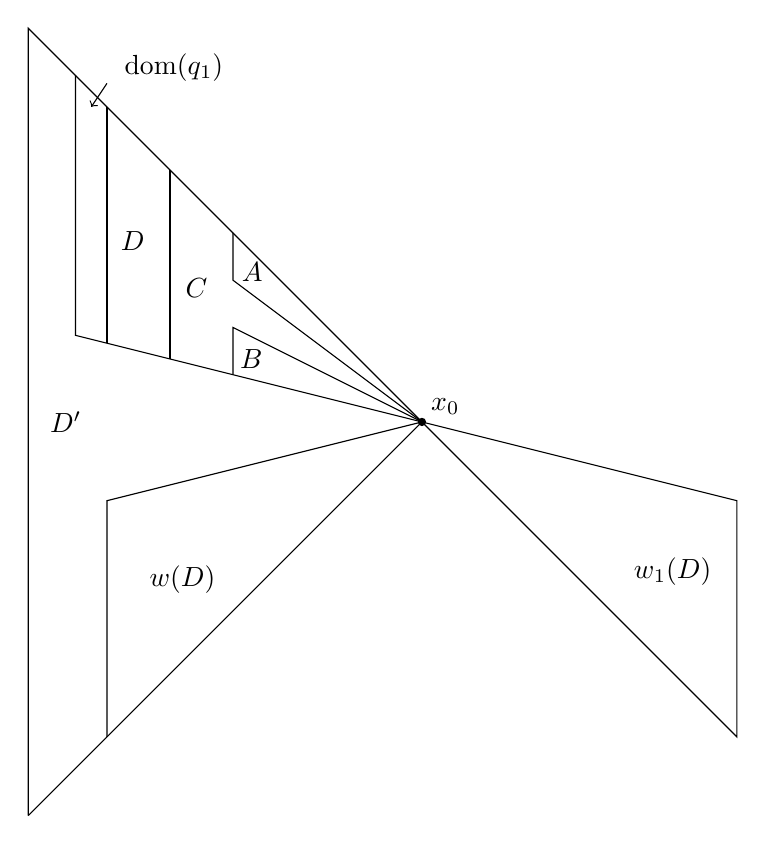
\begin{tikzpicture}[scale=0.1]

\draw (0,0) to (50,50) to (0,100) to (0,0);
\draw (10,10) to (10,40) to (50,50) to (90,40) to (90,10) to (50,50);
\draw (6, 94) to (6,61) to (50,50);
\draw (10, 60) to (10,90);
\draw (18, 58) to (18,82);
\draw (26, 56) to (26,62) to (50,50);
\draw (26, 74) to (26, 68) to (50,50);
\draw[->] (10,93) to (8,90);
\filldraw[fill=black, very thick] (50,50) circle (0.3);

\node[left] at (8, 50) {$D'$};
\node[left] at (25,30) {$w(D)$};
\node[left] at (88, 31) {$w_1(D)$};
\node[left] at (16, 73) {$D$};
\node[left] at (24, 67) {$C$};
\node[left] at (31, 69) {$A$};
\node[left] at (31, 58) {$B$};
\node[left] at (26,95) {$\mbox{dom}(q_1)$};
\node[left] at (56,52) {$x_0$};


\end{tikzpicture}
\caption{The composition of $D_1'$. \label{fig:1}}
\end{figure}
      
Extend the ordering on $D'$ to $D_1'$ so that the following hold:
    \begin{enumerate}
       \item[(a)] for any $y_1,y_2 \in D$, $w_1(y_1) < w_1(y_2)$ if and only if $w(y_1) < w(y_2)$;
       \item[(b)] for any $u \in A \cup B$ and $y \in D$, if $w(y) < b_n=\max(A\cup B)$, then $u<w_1(y)$ if and only if $u<w(y)$;
       \item[(c)] for any $y \in D$, if $w(y) > b_n$, then $a_n < w_1(y) <b_n$. 
    \end{enumerate}
    Such an extension clearly exists. 

Now define $g_1\colon A\cup w(D)\to A\cup w_1(D)$ by letting $g_1(a) = a$ for all $a\in A$ and $g_1(w(y)) = w_1(y)$ for all $y\in D$. Then $g_1$ is order-preserving by the above requirements (a) through (c). To see that $g_1$ is a partial isometry, let $a \in A$ and $y\in D$. Since $\mbox{dom}(q_1)\cup w(D)$ is the free amalgam of $\mbox{dom}(q_1)$ and $w(D)$ over $\{x_0\}$ and $D_1'$ is the free amalgam of $D'$ and $w_1(D)$ over $\{x_0\}$, we have \[d(a, w(y))=d(a,x_0)+d(x_0,w(y))=d(a,x_0)+d(x_0,w_1(y))=d(a,w_1(y)).\] 
    Intuitively, $g_1$ sends $w(y)$ to a copy which is smaller than $b_n$ and fixes $A$ pointwise. Consequently, we have $w_1(D)<b_n$ and, for any $y \in D$, $w_1(y) <x_0$ if and only if $w(y)<x_0$.
    
Let $w_2(D)$ be a fresh isomorphic copy of $w(D)$ such that $w_2(D)$ and $w(D)$ has exactly one common point $x_0$. Let $D_2'$ be the free amalgam of $D_1'$ and $w_2(D)$ over $\{x_0\}$. Extend the ordering on $D_1'$ to $D_2'$ so that the following hold:
 \begin{enumerate}
       \item[(d)] for any $y_1,y_2 \in D$, $w_2(y_1) < w_2(y_2)$ if and only if $w_1(y_1) < w_1(y_2)$;
       \item[(e)] for any $u \in A \cup B$ and $y \in D$, if $w(y) < a_n$, then $u<w_2(y)$ if and only if $u<w_1(y)$;
       \item[(f)] for any $y \in D$, if $w(y) > a_n$, then $b_{n-1} < w_2(y) <a_n$. 
    \end{enumerate}
Define an order-preserving partial isometry $g_2\colon B\cup w_1(D)\to B\cup w_2(D)$ by letting $g_2(b)=b$ for all $b\in B$ and $g_2(w_1(y))=w_2(y)$ for all $y\in D$. Moreover, $w_2(D) < a_n$ and, for any $y \in D$, $w_2(y) <x_0$ if and only if $w_1(y)<x_0$.
    
Repeating this construction, we obtain, for $1\leq i \leq 2n$, $D_i'=D' \cup w_1(D) \cup \dots \cup w_i(D)$, which can be viewed as the free amalgam of $w_i(D)$ and the remaining part over $\{x_0\}$, an ordering on $D_{2n}'$ extending that on $D'$, and order-preserving partial isometries $g_1, g_2, g_3, \dots,g_{2n}$ such that 
\begin{enumerate}
\item[(i)] for any $1\leq i\leq n$, $g_{2i-1}(a)=a$ for all $a\in A$, and $g_{2i}(b)=b$ for all $b\in B$;
\item[(ii)] for any $1\leq i\leq n$ and $y\in D$, $g_{2i}(w_{2i-1}(y))=w_{2i}(y)$, and $g_{2i-1}(w_{2i-2}(y))=w_{2i-1}(y)$ if $i>1$.
\end{enumerate}
Moreover, we have $w_{2n}(D) <a_1$ and, for any $y \in D$, $w_{2n}(y) <x_0$ if and only if $w(y)<x_0$. 

Define a map $$r\colon A\cup w_{2n}(C)\to A\cup w_{2n}(p(C))$$ by letting $r(a)=a$ for all $a\in A$ and $r(w_{2n}(c))=w_{2n}(p(c))$ for all $c\in C$. Then for $a \in A$ and $c \in C$,  we have
    \begin{align*}
    d(a,w_{2n}(c)) &=d(a,x_0)+d(x_0,w_{2n}(c))=d(a,x_0)+d(x_0,w(c))\\&=d(a,x_0)+d(x_0,c)=d(a,x_0)+d(x_0,p(c))\\&=d(a,x_0)+d(x_0,w(p(c))) \\
& =d(a,x_0)+d(x_0,w_{2n}(p(c)))=d(a,w_{2n}(p(c))) \\
&=d(r(a),r(w_{2n}(c))).
    \end{align*} 
Thus $r$ is a partial isometry. Note that $w$ and $p$ are order-preserving and each fixes $x_0$. Thus for any $c\in C$, we have 
    \begin{align*}
      w_{2n}(c)<x_0 &\iff w(c)<x_0 \iff c<x_0 \\&\iff p(c) <x_0 \iff w(p(c))<x_0 \\&\iff w_{2n}(p(c))<x_0. 
    \end{align*}
    Since for all $y \in D$, $w_{2n}(y)<a_1$, we conclude that $r$ is an order-preserving partial isometry. 



By Lemma~\ref{lemma:Extensions} and our construction, the distances in $D_{2n}'$ are all taken from the additive semigroup generated by the distances in $D$. Now redefine the metric on $D_{2n}'$ by taking the minimum of the original distance value and $\sup\Delta$. Call the resulting metric space $D''$. Since $D$ is a $\Delta$-metric space, it follows that $D''$ is a $\Delta$-metric space, and, as an ordered metric space, $D''$ is an extension of $D$. Moreover, each of the order-preserving partial isometries $q_1, q_2, g_1, g_2, \dots, g_{2n}, r$ continues to be order-preserving partial isometries of $D''$. 

Now by the weak homogeneity of $\mathbb{U}_{\Delta}^<$, we can extend $D$ to an isomorphic copy of $D''$ as a substructure of $\mathbb{U}_\Delta^<$. By the ultrahomogeneity of $\mathbb{U}_\Delta^<$, we can extend all the above order-preserving partial isometries to full automorphisms of $\mathbb{U}_{\Delta}^<$. Denote the resulting automorphisms by the same notation. Then for $1\leq i\leq 2n$, we have $r, q_1,g_i \in {\rm Aut}_A(\mathbb{U}_{\Delta}^<)$ if $i$ is odd, and $q_2,g_i \in {\rm Aut}_B(\mathbb{U}_{\Delta}^<)$ if $i$ is even. Finally, for any $c \in C$, \[p(c)=w(q_1,q_2)^{-1}g_1^{-1}\dots g_{2n}^{-1}rg_{2n}\dots g_1w(q_1,q_2)(c).\]
Thus if we let 
$$q=w(q_1,q_2)^{-1}g_1^{-1}\dots g_{2n}^{-1}rg_{2n}\dots g_1w(q_1,q_2), $$
then $q\in \langle {\rm Aut}_A(\mathbb{U}_\Delta^<), {\rm Aut}_B(\mathbb{U}_\Delta^<) \rangle$ and $p\upharpoonright C=q\upharpoonright C$ as required.
     \end{proof}

     \begin{lemma}\label{theorem:density}
        Let $\Delta$ be a countable distance value set, and let $A,B \subseteq \mathbb{U}_{\Delta}^<$ be finite subsets. Suppose $A \cap B = \varnothing$. Then \[\langle {\rm Aut}_A(\mathbb{U}_{\Delta}^<), {\rm Aut}_B(\mathbb{U}_{\Delta}^<) \rangle  \ is \ dense \ in \  {\rm Aut}(\mathbb{U}_{\Delta}^<).\]
\end{lemma}    

\begin{proof}   Let $p \in {\rm Aut}(\mathbb{U}_{\Delta}^<)$ and let $C \subseteq \mathbb{U}_{\Delta}^<$ be a finite subset. We show that there is a $q \in \langle {\rm Aut}_A(\mathbb{U}_{\Delta}^<), {\rm Aut}_B(\mathbb{U}_{\Delta}^<) \rangle$ such that $p\upharpoonright C=q\upharpoonright C$. Again we may assume $A\cup B \subseteq C$. Consider the ordered $\Delta$-metric space $C \cup p(C)$. Extend it to an ordered $\Delta$-metric space $C \cup p(C) \cup \{x_0\}$, where the metric is defined by 
$$d(x_0,y)=\mbox{diam}(C\cup p(C))=\max\{d(y_1,y_2)\colon y_1,y_2 \in C \cup p(C)\}$$
for any $y\in C\cup p(C)$, and the ordering is defined by $x_0 <y$ for all $y\in C\cup p(C)$.
           Such an extension can be found in $\mathbb{U}_{\Delta}^<$ by the weak homogeneity of $\mathbb{U}^<_\Delta$, and so we may assume $x_0 \in \mathbb{U}_{\Delta}^<$. Now consider $A' = A \cup \{x_0\}$, $B' = B \cup \{x_0\}$ and let $p' \in {\rm Aut}_{x_0}(\mathbb{U}_\Delta^<)$ be an extention of $p\upharpoonright C \cup \{(x_0,x_0)\}$. Applying Lemma~\ref{lemma:density} to $A', B'$ and $p'$, we get a $q \in \langle {\rm Aut}_{A'}(\mathbb{U}_{\Delta}^<), {\rm Aut}_{B'}(\mathbb{U}_{\Delta}^<) \rangle$ such that $q\upharpoonright C\cup\{x_0\}=p'\upharpoonright C\cup\{x_0\}$. Then in particular $q \in \langle {\rm Aut}_A(\mathbb{U}_{\Delta}^<), {\rm Aut}_B(\mathbb{U}_{\Delta}^<) \rangle$ and $q\upharpoonright C=p\upharpoonright C$ as required. 
        \end{proof}
 
We also need the following two lemmas about proper open subgroups of $\mbox{\rm Aut}(\mathbb{U}^<_\Delta)$.    

     \begin{lemma}\label{lemma:f_orbit}
        Let $V$ be a proper open subgroup of ${\rm Aut}(\mathbb{U}_{\Delta}^<)$. Then there exists an element $x \in \mathbb{U}_{\Delta}^<$ such that $V\cdot x$ is finite.
        \begin{proof}
           Toward a contradiction, assume $V\cdot x$ is infinite for all $x\in \mathbb{U}_{\Delta}^<$. We prove that $V$ is dense. Since $V$ is also closed, it follows that $V = {\rm Aut}(\mathbb{U}_{\Delta}^<)$, contradicting the properness of $V$. 

Note that a basic open neighborhood of the identity element of $\mbox{\rm Aut}(\mathbb{U}^<_\Delta)$ has the form ${\rm Aut}_{A}(\mathbb{U}_{\Delta}^<)$, where $A$ is a finite subset of $\mathbb{U}^<_\Delta$. Since $V$ is an open subgroup, there is a finite $A\subseteq \mathbb{U}^<_\Delta$ such that ${\rm Aut}_{A}(\mathbb{U}_{\Delta}^<) \subseteq V$. By Neumann's lemma (see Corollary 4.2.2 of Hodges \cite{Hodges}), there exists $g \in V$ such that $g(A)\cap A = \varnothing$. 
           
By Lemma~\ref{theorem:density}, $\langle {\rm Aut}_{A}(\mathbb{U}_{\Delta}^<), {\rm Aut}_{g(A)}(\mathbb{U}_{\Delta}^<) \rangle$ is dense in ${\rm Aut}(\mathbb{U}_{\Delta}^<)$. This group is contained in $V$, and thus $V$ is dense. 
        \end{proof}
     \end{lemma}

     %We use the following lemma to reconstruct $\mathbb{U}_\Delta^<$. 
     \begin{lemma}\label{lem:maxopen}
        Let $V$ be a proper open subgroup of ${\rm Aut}(\mathbb{U}_{\Delta}^<)$. The following are equivalent:
        \begin{enumerate}
           \item[\rm (1)] There exists a unique $x \in \mathbb{U}_{\Delta}^<$ such that $V = {\rm Aut}_{\{x\}}(\mathbb{U}_{\Delta}^<)$. 
           \item[\rm (2)] $V$ is maximal among proper closed subgroups of ${\rm Aut}(\mathbb{U}_{\Delta}^<)$. 
        \end{enumerate}
        \end{lemma}
\begin{proof}
           First suppose $V = {\rm Aut}_{\{x\}}(\mathbb{U}_{\Delta}^<)$. Assume $H$ is a closed subgroup of $\mbox{\rm Aut}(\mathbb{U}^<_\Delta)$ such that $V\subsetneq H\subsetneq \mbox{\rm Aut}(\mathbb{U}^<_\Delta)$.  Let $g \in H \setminus V$. Then $g(x) \neq x$ and ${\rm Aut}_{\{g(x)\}}(\mathbb{U}_{\Delta}^<) = g{\rm Aut}_{\{x\}}(\mathbb{U}_{\Delta}^<)g^{-1}=gVg^{-1} \leq H$. By Lemma~\ref{theorem:density}, $\langle {\rm Aut}_{\{g(x)\}}(\mathbb{U}_{\Delta}^<), {\rm Aut}_{\{x\}}(\mathbb{U}_{\Delta}^<) \rangle$ is dense in ${\rm Aut}(\mathbb{U}_{\Delta}^<)$. Since it is a subgroup of $H$ and $H$ is closed, we have $H= {\rm Aut}(\mathbb{U}_{\Delta}^<)$, contradicting the properness of $H$. 
     
           For the converse, assume (2) holds. By Lemma~\ref{lemma:f_orbit}, there exists an element $x \in \mathbb{U}_{\Delta}^<$ such that $V\cdot x$ is finite. We show that $V\subseteq \mbox{\rm Aut}_{\{x\}}(\mathbb{U}^<_\Delta)$. Otherwise, let $g \in V$ be such that $g(x) \neq x$. Then either $g(x)>x$ or $g(x)<x$. Since $g$ is order-preserving, we get that either $g^{n+1}(x) > g^n(x)$ for all natural numbers $n$, or $g^{n+1}(x)<g^n(x)$ for all natural numbers $n$. In either case, $V\cdot x$ is infinite. 
           
It is clear that $\mbox{\rm Aut}_{\{x\}}(\mathbb{U}^<_\Delta)\neq \mbox{\rm Aut}(\mathbb{U}^<_\Delta)$. Thus by the the maximality of $V$, we have
$V=\mbox{\rm Aut}_{\{x\}}(\mathbb{U}^<_\Delta)$.
     
           For the uniqueness, assume ${\rm Aut}_{\{x\}}(\mathbb{U}_{\Delta}^<) = {\rm Aut}_{\{y\}}(\mathbb{U}_{\Delta}^<)$ but $x \neq y$. Then by Lemma~\ref{theorem:density}, $\langle {\rm Aut}_{\{x\}}(\mathbb{U}_{\Delta}^<), {\rm Aut}_{\{y\}}(\mathbb{U}_{\Delta}^<) \rangle$ is dense. But $$\langle {\rm Aut}_{\{x\}}(\mathbb{U}_{\Delta}^<), {\rm Aut}_{\{y\}}(\mathbb{U}_{\Delta}^<) \rangle={\rm Aut}_{\{x\}}(\mathbb{U}_{\Delta}^<) = {\rm Aut}_{\{y\}}(\mathbb{U}_{\Delta}^<),$$ and thus they are both the whole group, which is impossible. 
        \end{proof}
     
     We are now ready to finish the proof of Theorem~\ref{thm:class}. Recall that the remaining direction is (i) implying (ii).

        Let $f\colon \mbox{\rm Aut}(\mathbb{U}^<_\Delta)\to\mbox{\rm Aut}(\mathbb{U}^<_\Lambda)$ be a topological group isomorphism. By Lemma~\ref{lem:maxopen}, for each $x \in \mathbb{U}_{\Delta}^<$, there is a unique $y \in \mathbb{U}_{\Lambda}^<$ such that $f({\rm Aut}_{\{x\}}(\mathbb{U}_{\Delta}^<))={\rm Aut}_{\{y\}}(\mathbb{U}_{\Lambda}^<)$. We write $y=g(x)$. The map $g$ is well-defined and bijective. 

        Note that for any $x,y,x',y'\in\mathbb{U}_{\Delta}^<$, ${\rm Aut}_{\{x,y\}}(\mathbb{U}_{\Delta}^<)$ and ${\rm Aut}_{\{x',y'\}}(\mathbb{U}_{\Delta}^<)$ are conjugate in $\mbox{\rm Aut}(\mathbb{U}^<_\Delta)$ if and only if $d(x,y)=d(x',y')$. Also note that
$$ {\rm Aut}_{\{x,y\}}(\mathbb{U}_{\Delta}^<)=\mbox{\rm Aut}_{\{x\}}(\mathbb{U}^<_\Delta)\cap \mbox{\rm Aut}_{\{y\}}(\mathbb{U}^<_\Delta) $$
and similarly for $\mbox{\rm Aut}_{\{x',y'\}}(\mathbb{U}^<_\Delta)$. Thus by the definition of $g$, we have that for any $x,y,x',y' \in \mathbb{U}_{\Delta}^<$,
$$ d(x,y)=d(x',y') \iff d(g(x),g(y)) = d(g(x'),g(y')).$$
        
Now for any $d \in \Delta$, we define $\theta(d) \in \Lambda$ by finding $x,y \in \mathbb{U}_{\Delta}^<$ such that $d(x,y)=d$, and then setting $\theta(d)=d(g(x),g(y))$. By the above observation, $\theta$ is well-defined and bijective. We show that $\theta$ witnesses the equivalence of $\Delta $ and $ \Lambda$. Suppose $(d_1,d_2,d_3)$ is a $\Delta$-triangle. There exist $x,y,z \in \mathbb{U}_{\Delta}^<$ such that the distances among them are exactly $(d_1,d_2,d_3)$. Then the distaces among $g(x),g(y),g(z)$ are $(\theta(d_1),\theta(d_2),\theta(d_3))$. Thus $(\theta(d_1),\theta(d_2),\theta(d_3))$ is a $\Lambda$-triangle. The converse also holds.

The proof of Theorem~\ref{thm:class} is complete.
    

     
     






















\section{The Complexity of the Equivalence between Distance Value Sets\label{sec:CDVS}}

In this section we study the complexity of the equivalence (see Definition~\ref{def:CDVSequiv}) between countable distance value sets from the point of view of descriptive set theory. We first establish some notation.

\begin{definition}
        Let $\mathsf{CDVS}\subseteq \mathbb{R}^{\mathbb{N}}$ consist of all sequences $(d_i)_{i\in\mathbb{N}}$ of real numbers such that
\begin{enumerate}
\item[(a)] $d_i\geq 0$ for all $i$; the set $\{i\in\mathbb{N}\colon d_i=0\}$ is infinite; $d_i>0$ for some $i$;
\item[(b)] if $d_i, d_j>0$, then $d_i=d_j$ if and only if $i=j$;
\item[(c)] if $\sup_kd_k<\infty$, then $\sup_k d_k=d_{i}$ for some $i$;
\item[(d)] for any $i,j\geq 0$, if $d_i+d_j<\sup_kd_k$ then there is $\ell$ such that $d_{\ell}=d_i+d_j$.
\end{enumerate}
\end{definition}

Intuitively, $\mathsf{CDVS}$ consists of codes of all countable distance value sets, which are enumerated as sequences of real numbers without repetitions. We include zero entries in the codes to accommodate finite distance value sets. $\mathsf{CDVS}$ is a Borel subset of $\mathbb{R}^{\mathbb{N}}$, and hence it is a standard Borel space. We also use the following notation:
$$\begin{array}{lcl}
\mathsf{CDVS}_0&=&\left\{(d_i)_{i\in\mathbb{N}}\in \mathsf{CDVS}\colon \inf\{d_i>0\colon i\in\mathbb{N}\}=0 \right\}, \\
\mathsf{CDVS}_+&=&\left\{(d_i)_{i\in\mathbb{N}}\in \mathsf{CDVS}\setminus \mathsf{CDVS}_0\colon \sup_i d_i<\infty\right\},\\
\mathsf{CDVS}_\infty &=& \left\{(d_i)_{i\in\mathbb{N}}\in \mathsf{CDVS}\setminus \mathsf{CDVS}_0\colon \sup_i d_i=\infty\right\}. 
\end{array}$$
These sets form a partition of $\mathsf{CDVS}$ into Borel subsets, and in particular they are all standard Borel spaces. $\mathsf{CDVS}_0$ consists of codes of all countable distance value sets $\Delta$ with $\inf\Delta=0$. Similarly, $\mathsf{CDVS}_+$ codes countable distance value sets $\Delta$ with $\inf\Delta>0$ and $\sup\Delta<\infty$, and $\mathsf{CDVS}_\infty$ codes those $\Delta$ with $\inf\Delta>0$ and $\sup\Delta=\infty$. In our discussions below, we will not distinguish a countable distance value set $\Delta$ from a code of $\Delta$ as an element of $\mathsf{CDVS}$.


\begin{definition}\label{def:er} %Let $\sim$ be the equivalence relation on $\mathbb{R}^{\mathbb{N}}$ defined by
%$$ (c_i)_i\sim (d_i)_i\iff \exists g\in S_\infty\ \exists r\in (0,+\infty)\ \forall i\ d_{g(i)}=r\cdot c_i. $$
Let $\approx$ be the equivalence relation on $\mathbb{R}^{\mathbb{N}}$ defined by
$$\begin{array}{rcl} (c_i)_i\approx (d_i)_i&\iff& \exists g\in S_\infty\ [\forall i\ (c_i=0\longleftrightarrow d_{g(i)}=0) \mbox{ and } \\
& & \forall i, j, k\ (|c_j-c_k|\leq c_i\leq c_j+c_k\longleftrightarrow \\
& & |d_{g(j)}-d_{g(k)}|\leq d_{g(i)}\leq d_{g(j)}+d_{g(k)})].
\end{array}
$$
For any $A\subseteq \mathbb{R}^{\mathbb{N}}$, %let $\sim_A$ denote $\sim\upharpoonright (A\times A)$, and similarly, 
let $\approx_A$ denote $\approx\upharpoonright (A\times A)$.
\end{definition}

Thus $\approx_{\mathsf{CDVS}}$ is the equivalence between countable distance value sets. Note that $\mathsf{CDVS}_0$, $\mathsf{CDVS}_+$ and $\mathsf{CDVS}_\infty$ are all invariant under the equivalence relation $\approx$. 

In the rest of this section we will determine the exact complexity of $\approx_{\mathsf{CDVS}_+}$, $\approx_{\mathsf{CDVS}_\infty}$ and $\approx_{\mathsf{CDVS}}$ and give some upper and lower bounds for $\approx_{\mathsf{CDVS}_0}$ in the Borel reducibility hierarchy.



\subsection{The exact complexity of $\approx_{\mathsf{CDVS}_+}$ and $\approx_{\mathsf{CDVS}}$}

\begin{lemma}\label{lem:isomorphism} $\approx_{\mathsf{CDVS}}$ is Borel reducible to an isomorphism relation of countable structures. Consequently, $\approx_{\mathsf{CDVS}}$ is Borel reducible to $E^\infty_{S_\infty}$.
\end{lemma}

\begin{proof} To each $\Delta\in \mathsf{CDVS}$ we associate a countable structure $\mathcal{A}_\Delta=(\Delta, R^{\mathcal{A}})$, where $R^{\mathcal{A}}$ is a ternary relation defined as
$$ R^{\mathcal{A}}(d_1,d_2,d_3)\iff \mbox{$(d_1,d_2,d_3)$ is a $\Delta$-triangle.}$$
It is clear that for $\Delta, \Lambda\in \mathsf{CDVS}$, we have $\Delta\approx \Lambda$ if and only if $\mathcal{A}_\Delta\cong \mathcal{A}_{\Lambda}$. This gives a Borel reduction from $\approx_{\mathsf{CDVS}}$ to an isomorphism relation of countable structures.
\end{proof}

\begin{theorem}\label{thm:CDVS+} The isomorphism relation of all countable linear orders is Borel reducible to $\approx_{\mathsf{CDVS}_+}$. Consequently, $E^\infty_{S_\infty}$ is Borel reducible to $\approx_{\mathsf{CDVS}_+}$.
\end{theorem}

\begin{proof}
For a countable linear order $\mathcal{O}$, let $\psi(\mathcal{O})\subseteq (3,4)$  be an isomorphic copy of $\mathcal{O}$, and let 
$$\varphi(\mathcal{O})=\{2,4,6\}\cup\psi(\mathcal{O})\cup(2+\psi(\mathcal{O})). $$
Then $\varphi(\mathcal{O})\in \mathsf{CDVS}_+$. We verify that $\varphi$ is a Borel reduction from the isomorphism relation of all countable linear orders to $\approx_{\mathsf{CDVS}_+}$.

First suppose $\mathcal{O}_1$ and $\mathcal{O}_2$ are isomorphic countable linear orders. Then there is an order-preserving bijection $f$ between $\psi(\mathcal{O}_1)$ and $\psi(\mathcal{O}_2)$. For $x\in\varphi(\mathcal{O}_1)$, let 
$$F(x)=\left\{\begin{array}{ll} f(x),  & \mbox{ if $x\in\psi(\mathcal{O}_1)$,} \\
f(x-2)+2, & \mbox{ if $x\in 2+\psi(\mathcal{O}_1)$,} \\
x, & \mbox{ otherwise.}
\end{array}\right.
$$
It is straightforward to check that $F$ is a bijection between $\varphi(\mathcal{O}_1)$ and $\varphi(\mathcal{O}_2)$ witnessing their equivalence. Thus $\varphi(\mathcal{O}_1)\approx \varphi(\mathcal{O}_2)$.

Conversely, suppose $\varphi(\mathcal{O}_1)\approx \varphi(\mathcal{O}_2)$ and this equivalence is witnessed by a bijection $g$. Let $\Delta=\varphi(\mathcal{O}_1)$ and $\Lambda=\varphi(\mathcal{O}_2)$, and let $\mathcal{A}_\Delta=(\Delta, R^\Delta)$ and $\mathcal{A}_\Lambda=(\Lambda, R^\Lambda)$ be the countable structures defined in the proof of Lemma~\ref{lem:isomorphism}.  Then $g$ is an isomorphism witnessing $\mathcal{A}_\Delta\cong \mathcal{A}_\Lambda$. 

Now note that $2$ is definable in both $\mathcal{A}_\Delta$ and $\mathcal{A}_\Lambda$ by the formula $\exists y\neg R(x, x, y)$. Thus $g(2)=2$. 
Moreover, $\psi(\mathcal{O}_1)$ is definable in $\mathcal{A}_\Delta$ by the formula 
$$ x\neq 2\wedge R(2, 2, x) \wedge \exists y\neg R(2,x,y). $$
Similarly, $\psi(\mathcal{O}_2)$ is definable in $\mathcal{A}_\Lambda$ by the same formula. Thus $g$ sends $\psi(\mathcal{O}_1)$ to $\psi(\mathcal{O}_2)$. Finally, on $\psi(\mathcal{O}_1)$, the $x<y$ relation is definable by the formula
$$ \exists z\, [\neg R(2, x, z) \wedge R(2,y,z)]. $$
Similarly for $\psi(\mathcal{O}_2)$. Hence $g$ preserves the order $<$ as a bijection between $\psi(\mathcal{O}_1)$ and $\psi(\mathcal{O}_2)$. It follows that the linear orders $\mathcal{O}_1$ and $\mathcal{O}_2$ are isomorphic.

It is routine to check that $\varphi$ is Borel.
\end{proof}

\begin{corollary}\label{cor:main} Both $\approx_{\mathsf{CDVS}_+}$ and $\approx_{\mathsf{CDVS}}$ are Borel bireducible with $E^\infty_{S_\infty}$. In particular, they are analytic and non-Borel.
\end{corollary}

\begin{proof} This follows immediately from Lemma~\ref{lem:isomorphism} and Theorem~\ref{thm:CDVS+}, in view of the trivial fact that $\approx_{\mathsf{CDVS}_+}$ is Borel reducible to $\approx_{\mathsf{CDVS}}$ via the identity function.
\end{proof}


\subsection{The exact complexity of $\approx_{\mathsf{CDVS}_\infty}$}

\begin{theorem}\label{thm:CDVSinfty} Let $\Delta$ and $\Lambda$ be countable distance value sets with $\inf\Delta=\inf\Lambda=1$ and $\sup\Delta=\sup\Lambda=\infty$. Then $\Delta$ and $\Lambda$ are equivalent if and only if $\Delta=\Lambda$.
\end{theorem}

\begin{proof} The implication $\Leftarrow$ is obvious. We only show the $\Rightarrow$ direction. For this, let $f$ be a bijection between $\Delta$ and $\Lambda$ witnessing their equivalence. 

For a subset $I\subseteq \mathbb{R}$, let $\Delta_I=\Delta\cap I$ and $\Lambda_I=\Lambda\cap I$. Let $\mathcal{A}_\Delta=(\Delta, R^\Delta)$ and $\mathcal{A}_\Lambda=(\Lambda, R^\Lambda)$ be the countable structures defined in the proof of Lemma~\ref{lem:isomorphism}. Then $f$ is an isomorphism witnessing $\mathcal{A}_\Delta\cong \mathcal{A}_\Lambda$. 

First note that $\inf\Delta=1\in \Delta$ if and only if $\mathcal{A}_\Delta$ satisfies the sentence
$$ \exists x\, \forall y\, [ R(x, x, y)\rightarrow \forall z\, R(z, z, y)]. $$
Similarly for $\Lambda$. Thus $1\in \Delta$ if and only if $1\in \Lambda$. We consider two cases.

{\sc Case 1}: $1\in \Delta\cap \Lambda$. Since $\Delta$ and $\Lambda$ are distance value sets with $\sup\Delta=\inf\Delta=\infty$, we have that $k\in \Delta\cap \Lambda$ for all positive integers $k$. Note that $1$ is definable in $\mathcal{A}_\Delta$ by the formula
$$ \chi_1(x)=\forall y\, [ R(x, x, y)\rightarrow \forall z\, R(z, z, y)]. $$
Similarly for $\mathcal{A}_\Lambda$. Thus $f(1)=1$. Also, we have that $\Delta_{[1,2]}$ is definable in $\mathcal{A}_\Delta$ by the formula
$$ \chi_{[1,2]}(x)=\forall y\, R(y,y,x). $$
Similarly for $\Lambda_{[1,2]}$. Hence $f$ sends $\Delta_{[1,2]}$ to $\Lambda_{[1,2]}$. 

Now for $k\geq 2$, define inductively 
$$ \chi_{[1,k+1]}(x)=\exists y\, [\chi_{[1,k]}(y)\wedge R(1,y,x)]. $$
Then $\Delta_{[1,k+1]}$ is definable in $\mathcal{A}_\Delta$ by $\chi_{[1,k+1]}$, and similarly for $\Lambda_{[1,k+1]}$. It follows that $f$ sends $\Delta_{[1,k+1]}$ to $\Lambda_{[1,k+1]}$ for all $k\geq 1$.

Next we define, by induction on $k\in\mathbb{N}^+$ and $m\in\mathbb{N}$, a formula $\chi_{[1,1+\frac{k}{2^m}]}$ as follows.
$$\begin{array}{rcl} \chi_{[1, 1+\frac{k}{2^0}]}(x)&=&\chi_{[1, k+1]}(x) \mbox{ for all $k\geq 1$,} \\
\chi_{[1,1+\frac{k}{2^{m+1}}]}(x)&=& \forall y\, [R(x,x,y)\rightarrow \chi_{[1,1+\frac{k+2^m}{2^m}]}(y)].
\end{array}
$$
For any $k\in\mathbb{N}^+$ and $m\in\mathbb{N}$, the formula $\chi_{[1, 1+\frac{k}{2^m}]}$ defines $\Delta_{[1,1+\frac{k}{2^m}]}$ in $\mathcal{A}_\Delta$ and $\Lambda_{[1,1+\frac{k}{2^m}]}$ in $\mathcal{A}_\Lambda$. Hence $f$ sends $\Delta_{[1,1+\frac{k}{2^m}]}$ to $\Lambda_{[1,1+\frac{k}{2^m}]}$. This implies that for any dyadic rationals $1<a<b$, $f$ sends $\Delta_{[a,b]}$ to $\Lambda_{[a,b]}$. Hence $f$ must be the identity function, and so $\Delta=\Lambda$.

{\sc Case 2}: $1\not\in \Delta\cup\Lambda$. The formula $\chi_{[1,2]}$ now defines $\Delta_{(1,2]}$ in $\mathcal{A}_\Delta$ and $\Lambda_{(1,2]}$ in $\mathcal{A}_\Lambda$. Thus $f$ sends $\Delta_{(1,2]}$ to $\Lambda_{(1,2]}$. 

Let
$$ \varphi_2(x)=\exists y\, [\chi_{[1,2]}(y)\wedge\forall z\,(\chi_{[1,2]}(z)\rightarrow R(x,y,z))]\wedge \neg \chi_{[1,2]}(x) $$
and let $D_2$ be defined by $\varphi_2$ in $\mathcal{A}_\Delta$. Then $D_2\subseteq\Delta_{(2,3]}$. We claim that $D_2\neq \varnothing$.  To see this, let $a, b\in \Delta_{(1,2]}$ be such that $a<b$ and $2(a-1)<b-1$. Such $a, b$ exist since $\inf\Delta=1\not\in \Delta$.  Then $2a\in\Delta$ since $\Delta$ is a distance value set, and $\varphi_2[2a]$ holds in $\mathcal{A}_\Delta$ as witnessed by $b$. Thus $2a\in D_2$. A similar argument shows $\inf D_2=2$. It follows that $\Delta_{(2,3]}$ is definable in $\mathcal{A}_\Delta$ by the formula
$$ \chi_{(2,3]}(x)=\forall y\, \forall z\, [(\chi_{[1,2]}(y)\wedge \varphi_2(z))\rightarrow R(x,y,z)]\wedge \neg\chi_{[1,2]}(x) $$
and $\Delta_{(1,3]}$ is definable in $\mathcal{A}_\Delta$ by the formula
$$ \chi_{(1,3]}(x)=\chi_{[1,2]}(x)\vee \chi_{(2,3]}(x). $$
Similarly for $\mathcal{A}_\Lambda$. Therefore $f$ sends $\Delta_{(2,3]}$ to $\Lambda_{(2,3]}$ and sends $\Delta_{(1,3]}$ to $\Lambda_{(1,3]}$.

Now for $k\geq 2$, define inductively
$$\begin{array}{rcl} \varphi_{k+1}(x)&=&\exists y\, [\varphi_k(y) \wedge \forall z\, (\chi_{[1,2]}(z)\rightarrow R(x,y,z))]\wedge \neg\chi_{(1,k+1]}(x), \\
\chi_{(k+1,k+2]}(x)&=&\forall y\, \forall z\, [(\chi_{[1,2]}(y)\wedge \varphi_{k+1}(z))\rightarrow R(x,y,z)]\wedge \neg\chi_{(1,k+1]}(x), \\
\chi_{(1,k+2]}(x)&=& \chi_{(1,k+1]}(x)\vee \chi_{(k+1,k+2]}(x). 
\end{array} $$ 
Then for all $k\geq 1$, $\chi_{(1,k+2]}$ defines $\Delta_{(1,k+2]}$ in $\mathcal{A}_\Delta$ and $\Lambda_{(1,k+2]}$ in $\mathcal{A}_\Lambda$. Hence for all $k\geq 2$, $f$ sends $\Delta_{(1,k+1]}$ to $\Lambda_{(1,k+1]}$. 

The rest of the proof is similar to Case 1. We conclude that $f$ must be the identity function, and so $\Delta=\Lambda$.
\end{proof}



\begin{theorem} $\approx_{\mathsf{CDVS}_\infty}$ is Borel bireducible with $=^+$.
\end{theorem}

\begin{proof}
To each $\Delta\in \mathsf{CDVS}_\infty$ we associate a code for 
$$ \Delta^*=\displaystyle\frac{\Delta}{\inf\Delta}. $$
Then $\Delta^*\in \mathsf{CDVS}_\infty$ and $\inf\Delta^*=1$. By Theorem~\ref{thm:CDVSinfty}, the map $\Delta\mapsto \Delta^*$ is a Borel function witnessing that $\approx_{\mathsf{CDVS}_\infty}\,\leq_B\ =^+$.

Conversely, given any nonempty countable subset $A$ of the interval $(0,1)$, let $\Delta_A$ be the subsemigroup of $(\mathbb{R}^+,+)$ generated by $\{1\}\cup (1+A)$. Then $\Delta_A$ is a countable distance value set with $\inf \Delta_A= 1$ and $\sup\Delta_A=\infty$.  Thus $\Delta_A\in \mathsf{CDVS}_\infty$. Moreover, $\Delta_A\cap (1,2)=1+A$. By Theorem~\ref{thm:CDVSinfty}, if $A$ and $B$ are two nonempty countable subsets of $(0,1)$, then $\Delta_A$ and $\Delta_B$ are equivalent if and only if $\Delta_A=\Delta_B$, if and only if $1+A=1+B$, and if and only if $A=B$. Thus $A\mapsto \Delta_A$ is a Borel function witnessing that $=^+\,\leq_B\ \approx_{\mathsf{CDVS}_\infty}$.
\end{proof}











\subsection{The complexity of $\approx_{\mathsf{CDVS}_0}$\label{sec:4}} 



In this subsection we give some upper and lower bounds for the complexity of $\approx_{\mathsf{CDVS}_0}$. We also discuss some related equivalence relations. 

 \begin{theorem}\label{thm:simapprox}
        Let $\Delta$ and $\Lambda$ be countable distance value sets with $\inf\Delta=\inf\Lambda=0$. Then the following are equivalent: 
        \begin{enumerate}
            \item[\rm (1)] $\Delta$ and $\Lambda$ are equivalent. 
            \item[\rm (2)] There is a positive real number $r$ such that $\Lambda = r \cdot \Delta$. 
        \end{enumerate} 

        Moreover, if $\Delta$ and $\Lambda$ are equivalent, then every witness of their equivalence has the form of multiplication by a positive real number. 
     \end{theorem}
     
\begin{proof} The implication (2)$\Rightarrow$(1) is obvious. We only prove (1)$\Rightarrow$(2). For this, let $f$ be a bijection between $\Delta$ and $\Lambda$ witnessing their equivalence. Let $\mathcal{A}_\Delta=(\Delta, R^\Delta)$ and $\mathcal{A}_\Lambda$ be the countable structures defined in the proof of Lemma~\ref{lem:isomorphism}. Then $f$ is an isomorphism witnessing $\mathcal{A}_\Delta\cong \mathcal{A}_\Lambda$. Since $\Delta$ is a distance value set and $\inf\Delta=0$, we have that $\Delta$ is dense in $(0, \sup\Delta)$. Similarly, $\Lambda$ is dense in $(0, \sup\Lambda)$.

Fix a sequence $(\delta_i)_{i\in\mathbb{N}}$ in $\Delta$ such that $\delta_{i+1} < {\delta_i}/{2}$ for all $i$. Such a sequence exists since $\mathcal{A}_\Delta$ satisfies the sentence $\forall x\,\exists y\,\neg R(y,y,x)$. Since $f$ is an isomorphism, we have $f(\delta_{i+1})<{f(\delta_i)}/{2}$ for all $i$. 

We claim that $f$ is continuous as a function from $\Delta\subseteq\mathbb{R}$ to $\Lambda\subseteq\mathbb{R}$. To see this,  
fix $x \in \Delta$. For any $\epsilon > 0$, find an $i$ such that $\delta_i < x$ and $f(\delta_i) < \epsilon$. For any $y \in \Delta$ with $|x - y| < \delta_i$, $(x,y,\delta_i)$ is a $\Delta$-triangle. Thus $(f(x), f(y),f(\delta_i))$ is a $\Lambda$-triangle. In particular, $|f(x)-f(y)|<f(\delta_i)<\epsilon$. The actually proves that for all positive $\delta$, $f$ is uniformly continuous on $\Delta_{>\delta}\triangleq \Delta\cap (\delta,+\infty)$. 

Next we show that $f$ is in fact linear. In the proof we use notation such as $\Delta_{>\delta}$, $\Delta_{<\delta}$, and $\Delta_{[a,b]}$ with obvious meanings.

     
     %  If $x,y, x+y \in\Delta$, then $f(x+y) = f(x)+f(y)$. 
   
To show that $f$ is linear, assume $x,y,x+y\in \Delta$. We claim that
\begin{enumerate}
\item[(a)] $f(\Delta_{[|x-y|, x+y]}) \subseteq \Lambda_{[|f(x)-f(y)|, f(x)+f(y)]}$; 
\item[(b)] $f(\Delta_{>x+y}) \subseteq \Lambda_{>f(x)+f(y)}  \mbox{ or } f(\Delta_{>x+y})\subseteq \Lambda_{<|f(x)-f(y)|}$;
\item[(c)] $f(\Delta_{<|x-y|}) \subseteq \Lambda_{>f(x)+f(y)} \mbox{ or } f(\Delta_{<|x-y|})\subseteq \Lambda_{<|f(x)-f(y)|}$. 
\end{enumerate}
Let $z\in \Delta$. (a) is equivalent to saying that if $(x,y,z)$ is a $\Delta$-triangle, then $(f(x), f(y), f(z))$ is a $\Lambda$-triangle, which is immediate from our assumption. Also immediate is that if $z > x+y$, then $(x,y,z)$ is not a $\Delta$-triangle. Thus $(f(x),f(y),f(z))$ is not a $\Lambda$-triangle, and so either $f(z) > f(x)+f(y)$ or $f(z) < |f(x)-f(y)|$. Similarly for $z <|x-y|$. Now, to prove (b), assume toward a contradiction that there are $z_1, z_2\in \Delta$ with $z_1, z_2 >x+y$ such that $f(z_1)<|f(x)-f(y)|$ and $f(z_2)>f(x)+f(y)$. Without loss of generality assume $z_1<z_2$ (the argument for the case $z_1>z_2$ is similar). By the continuity of $f$ and the density of both $\Delta$ and $\Lambda$, we may find $z_1=a_1,\dots, a_n=z_2$ in $\Delta$ such that $a_k>x+y$ and $|f(a_{k+1})-f(a_k)| < f(x)+f(y)-|f(x)-f(y)|$ for all $1\leq k\leq n$. Then there must be an $a_k$ with $|f(x)-f(y)| \leq f(a_k) \leq f(x)+f(y)$, contradicting $a_k>x+y$. This proves (b). A similar argument for $z_1, z_2 < |x-y|$ proves (c). 

        Since $f$ is a bijection from $\Delta$ to $\Lambda$, the claimed inclusions are actually equalities. By considering sufficiently small $\delta_i$, we see that $f(\Delta_{<|x-y|}) = \Lambda_{<|f(x)-f(y)|}$, and thus $f(\Delta_{>x+y}) = \Lambda_{>f(x)+f(y)}$. By the continuty of $f$ again, we have $f(x+y) =f(x)+f(y)$.   
   
Finally, we argue that for any $x,t \in \Delta$, we have $f(x)/x=f(t)/t$. This proves (2). 


    For each $k > 0 $, find $0< \delta_k < 1/2^k$ by the continuity of $f$ such that for all $z\in \Delta$, $|t-z|<\delta_k$ implies $|f(t)-f(z)| < 1/k$. Now for each $k$, find positive rational number $n_k/m_k$ such that $0< t-(n_k/m_k)x < \delta_k/2$. Note that by the density of $\Delta$ and bijectivity of $f$, $\delta_k \to 0$ as $k \to \infty$. Thus $n_k/m_k \to t/x$ as $k \to \infty$. 

    Fix $k$. By the density of $\Delta$, find an increasing sequence $(t_j)_{j\in \mathbb{N}}$ with $t_j \in \Delta$ and $t_j \to x/m_k$ as $j \to\infty$. Then $m_kt_j \to x$ as $j \to \infty$, and $m_kt_j < x \in \Delta$. Thus $m_kt_j\in \Delta$ and $m_kf(t_j)=f(m_kt_j) \to f(x)$, which gives $f(t_j) \to f(x)/m_k$. On the other hand, $n_kt_j < (n_k/m_k)x < t \in \Delta$ and $n_kt_j \to (n_k/m_k)x$ as $j\to\infty$. Hence $n_kt_j\in \Delta$ and $f(n_kt_j)=n_kf(t_j) \to (n_k/m_k)f(x)$ as $j \to \infty$. 
    Thus we can find a $j$ such that $|n_kt_j-(n_k/m_k)x|<\delta_k/2$ and $|f(n_kt_j)-(n_k/m_k)f(x)|<1/k$. For this fixed $j$, we have $|t-n_kt_j|\leq |t-(n_k/m_k)x|+|n_kt_j-(n_k/m_k)x|<\delta_k$. Thus $|f(t)-f(n_kt_j)|<1/k$, and consequently $|f(t)-(n_k/m_k)f(x)|<2/k$. 

    Letting $k \to \infty$, we get $f(t)=(t/x)f(x)$ and thus $f(x)/x=f(t)/t$. 
\end{proof}



    

%Theorem 4.5 is a generalization of a result of Hion \cite{Hion} about Achimedean ordered groups.

   
     
     
     In view of Theorem~\ref{thm:simapprox}, we define the following notion.
\begin{definition}\label{def:er2} Let $\sim$ be the equivalence relation on $\mathbb{R}^{\mathbb{N}}$ defined by
$$ (c_i)_i\sim (d_i)_i\iff \exists g\in S_\infty\ \exists r\in (0,+\infty)\ \forall i\ d_{g(i)}=r\cdot c_i. $$
For any $A\subseteq \mathbb{R}^{\mathbb{N}}$, let $\sim_A$ denote $\sim\upharpoonright (A\times A)$.
\end{definition}

Thus Theorem~\ref{thm:simapprox} can be restated as
$\sim_{\mathsf{CDVS}_0}\,=\ \approx_{\mathsf{CDVS}_0}$. 

To obtain some upper and lower bounds for $\sim_{\mathsf{CDVS}_0}$ in the Borel reducibility hierarchy, we consider another equivalence relation defined and studied by Calderoni--Marker--Motto Ros--Shani \cite{CMMRS}. Let $\mathsf{ArGp}$ be the space of all countable Archimedean ordered groups, and let $\cong_{\mathsf{ArGp}}$ denote the isomorphism relation on $\mathsf{ArGp}$. It was proved in \cite{CMMRS} that
$$ =^+\ <_B\ \cong_{\mathsf{ArGp}}\ \leq_B\ \cong^*_{3,1}. $$
Here we prove the following facts.

\begin{lemma}\label{lem:argp} $\cong_{\mathsf{ArGp}}\ \leq_B\ \sim_{\mathsf{CDVS}_0}$.
\end{lemma}

\begin{proof} By a theorem of H\"{o}lder (see Theorem~2.1 of \cite{CMMRS}), every element of $\mathsf{ArGp}$ is isomorphic to a subgroup of $\mathbb{R}$ with the natural order of real numbers. Thus we may regard $\mathsf{ArGp}$ as the space of all countable subgroups of $\mathbb{R}$ with the natural order. Note that if $G\in \mathsf{ArGp}$ and $\inf [G\cap (0,+\infty)]\neq 0$, then $G$ is isomorphic to $\mathbb{Z}$. Let $\mathsf{ArGp}_0$ be the space of all elements of $\mathsf{ArGp}$ which are not isomorphic to $\mathbb{Z}$. Then $\mathsf{ArGp}\setminus\mathsf{ArGp}_0$ consists of exactly one isomorphism class of $\mathsf{ArGp}$, and it follows easily that $\cong_{\mathsf{ArGp}}\ \leq_B\  \cong_{\mathsf{ArGp}_0}$. 

For each $G\in\mathsf{ArGp}_0$, let $\Delta(G)=G\cap(0,+\infty)$. Then $\Delta(G)$ is a countable distance value set and $\inf \Delta(G)=0$. It is easy to see that $\Delta\colon \mathsf{ArGp}_0\to \mathsf{CDVS}_0$ is a Borel map. 

To see that $\Delta$ is a Borel reduction witnessing $\cong_{\mathsf{ArGp}}\ \leq_B\ \sim_{\mathsf{CDVS}_0}$, we use a result of Hion (see Lemma~2.2 of \cite{CMMRS}) which states that for any $G, H\in \mathsf{ArGp}$, $G\cong H$ if and only if there is a real number $r$ such that $r\cdot G=H$. It is then clear that $G\cong H$ if and only if there is a positive real number $r$ such that $r\cdot G=H$, if and only if there is a positive real number $r$ such that $r\cdot \Delta(G)=\Delta(H)$, and if and only if $\Delta(G)\sim \Delta(H)$.
\end{proof}


\begin{theorem}\label{thm:cong31} $\sim_{\mathsf{CDVS}_0}\ \leq_B\ \cong^*_{3,1}$.
\end{theorem}

\begin{proof}
    Similar to Proposition 3.12 of \cite{CMMRS}, using Corollary 6.4 of \cite{HKL}, this can be proved by showing that $\sim_{\mathsf{CDVS}_0}$ is Borel bireducible with an isomorphism relation and it is itself ${\bf\Sigma}^0_4$. 

We first show that $\sim$ is ${\bf\Sigma}^0_4$. For this, only note that for any $(c_i)_i, (d_i)_i\in \mathbb{R}^{\mathbb{N}}$, 
$$\begin{array}{rcl}
(c_i)_i\sim (d_i)_i&\iff& \exists i,j\ \left( c_i/d_j>0 \mbox{ and }\right. \\
& &  \forall n\ \exists m\ \left( c_n=d_mc_i/d_j \right) \mbox{ and }  \\
& &\left.\forall m\ \exists n\ \left( c_n=d_mc_i/d_j \right) \right). 
\end{array}$$

Next we show that $\sim_{\mathsf{CDVS}_0}$ is Borel bireducible with an isomorphism relation. For this we define a language $\mathcal{L}$ and an $\mathcal{L}_{\omega_1 \omega}$-theory $T$ so that the isomorphism relation on all countable models of $T$ is Borel bireducible with $\sim_{\mathsf{CDVS}_0}$.

    Let 
$$\mathcal{L}=\{0, c, \leq, +\}\cup\{R_q\colon q\in \mathbb{Q}^+\}$$
where 
\begin{itemize}
\item $0,c$ are constant symbols; 
\item $\leq$ is a binary relation symbol;
\item $+$ is a binary function symbol;
\item for each positive rational number $q\in \mathbb{Q}^+$, $R_q$ is a binary relation symbol.
\end{itemize}

In a countable distance value set $\Delta$ with $\inf\Delta=0$, we interpret $c$ to be $0$ if $\sup\Delta=+\infty$ and to be $\sup\Delta$ otherwise. For each $q\in \mathbb{Q}^+$, $R_q$ is interpreted as $R_q(x,y)$ if and only if $q<x/y$. Under these interpretations, $\Delta\cup\{0\}$ becomes a countable $\mathcal{L}$-structure.

 Let $T$ be an $\mathcal{L}_{\omega_1\omega}$-theory describing the following properties of a countable $\mathcal{L}$-structure $\mathcal{M}$ (for notational simplicity, we omit the superscripts $\mathcal{M}$ in the interpretations of the symbols of $\mathcal{L}$ in $\mathcal{M}$):
    \begin{enumerate}
        \item For all $q \in \mathbb{Q}^+$ and $x \in |\mathcal{M}|$, $\lnot R_q(x,0)$ and $\lnot R_q(0,x)$. 
        \item For all $x,y\in |\mathcal{M}|\setminus\{0\}$, the set of $q\in \mathbb{Q}^+$ with $R_q(x,y)$ is nonempty and forms a Dedekind cut of positive rational numbers, i.e., it is not the whole positive rational numbers, is closed downward and has no maximum. Moreover, the real number defined by the Dedekind cut $\{q \in \mathbb{Q}^+\colon R_q(x,x)\}$ is $1$. 
        \item For all $x,x',y \in |\mathcal{M}|\setminus\{0\}$, if $x\neq x'$, then the Dedekind cuts defined by $x,y$ and $x',y$ are different. 
        \item For all $x,y,z \in |\mathcal{M}|\setminus\{0\}$ and $p,q \in \mathbb{Q}^+$, if $R_p(x,y)$ and $R_q(y,z)$, then $R_{pq}(x,z)$, and if $\lnot R_p(x,y)$ and $\lnot R_q(y,z)$, then $\lnot R_{pq}(x,z)$. 
        \item $\leq$ is a linear ordering of $|\mathcal{M}|$,  $0$ is the $\leq$-least element, and for all $x,x'\in |\mathcal{M}|\setminus\{0\}$, $x \leq x'$ if and only if $x = x'$ or $R_1(x',x)$. 
        \item For all $x,x',y \in |\mathcal{M}|\setminus\{0\}$ and $q \in \mathbb{Q}^+$, $R_q(x+x',y)$ if and only if there are $q_1,q_2\in\mathbb{Q}^+$ with $q_1+q_2=q$ such that $R_{q_1}(x,y)$ and $R_{q_2}(x',y)$. 
        \item For all $x \in |\mathcal{M}|\setminus\{0\}$ and $q \in \mathbb{Q}^+$, there is $x' \in |\mathcal{M}|\setminus\{0\}$ such that $\lnot R_q(x',x)$. 
    \end{enumerate}
Let $\mbox{Mod}(T)$ denote the Borel class of all countable models of $T$. Let $\cong_T$ denote the isomorphism relation on $\mbox{Mod}(T)$. It remains to verify that both $\sim_{\mathsf{CDVS}_0}\ \leq_B\ \cong_T$ and $\cong_T\ \leq_B\  \sim_{\mathsf{CDVS}_0}$ hold. 

Let $\Delta$ be a countable distance value set with $\inf\Delta=0$. We define a countable $\mathcal{L}$-structure $\mathcal{M}_\Delta$. Let $\mathbb{R}^+$ denote the semigroup of positive real numbers. Let $\bar{\Delta}\subseteq \mathbb{R}^+$ be the sub-semigroup of $\mathbb{R}^+$ generated by $\Delta$. Then either $\Delta = \bar{\Delta}$ or $\Delta = \bar{\Delta} \cap (0,{\rm sup}\Delta]$. 
Let $|\mathcal{M}_\Delta| = \{0\} \cup \bar{\Delta}$. Define $0, \leq, +$ in the obvious way. For $q \in \mathbb{Q}^+$ and $x,y \in |\mathcal{M}_\Delta|$, if  either $x=0$ or $y=0$, then $\lnot R_q(x,y)$; otherwise, define $R_q(x,y)$ if and only if $q < x/y$. Finally, if $\sup\Delta=+\infty$, set $c = 0$; otherwise, set $c = {\rm sup}\Delta$. Now it is easy to verify that $\mathcal{M}_\Delta$ is a model of $T$. Note that clause (7) holds since $\Delta$ is dense in $(0, \sup\Delta)$.  It is also clear that the map $\Delta \mapsto \mathcal{M}_\Delta$ gives a Borel reduction from $\sim_{\mathsf{CDVS}_0}$ to $\cong_T$.  

    Now given a countable model $\mathcal{M} $ of $T$, we define a map $f:\mathcal{M} \to [0,+\infty)$ as follows. We first choose a non-zero element $y_0\in \mathcal{M}$ canonically. Then define $f(0)=0$, and for $x\neq 0$, let $f(x)$ be the positive real number defined by the Dedekind cut $\{q\in \mathbb{Q}^+ \colon R_q(x,y_0)\}$. By clauses (2) and (3), $f$ is an injection. Let $\Delta_{\mathcal{M}}$ be $f(\mathcal{M}) \setminus \{0\}$ if $c=0$ and $f(\mathcal{M}) \cap (0,f(c)]$ otherwise. 

By clause (7), we have $\inf\Delta_{\mathcal{M}}=0$. Thus to verify that $\Delta_{\mathcal{M}}$ is a countable distance value set, it suffices to check that $f(\mathcal{M})$ is closed under summation. For this just note that if $x,y \in \mathcal{M}$ are nonzero, then
    \begin{align*}
        q<f(x+y)&\iff R_q(x+y, y_0) \\& \iff \exists q_1,q_2 \ q_1+q_2=q \land R_{q_1}(x, y_0)\land R_{q_2}(y, y_0) \\& \iff \exists q_1,q_2 \ q_1+q_2=q \land q_1< f(x)\land q_2<f(y) \\& \iff q <f(x)+f(y).
    \end{align*}
    Thus we have $f(x+y)=f(x)+f(y)$, and so $f(\mathcal{M})$ is closed under summation. 

 Finally, we verify that the map $\mathcal{M}\mapsto \Delta_{\mathcal{M}}$ is a Borel reduction from $\cong_T$ to $\sim_{\mathsf{CDVS}_0}$.  It is clear that the map is Borel. For the reduction, we first claim that for nonzero $x,y \in \mathcal{M}$, $R_q(x,y)$ if and only if $q<f(x)/f(y)$. Suppose $R_q(x,y)$. There is $q'>q$ with $R_{q'}(x,y)$.  Let $p<q'f(y)$. Then $p/q' <f(y)$ and thus $R_{p/q'}(y,y_0)$. Since $R_{q'}(x,y)$, by clause (4), we have $R_p(x,y_0)$ and thus $p<f(x)$. This shows $q'\leq f(x)/f(y)$ and thus $q <f(x)/f(y)$. Similarly we can prove that if $\lnot R_q(x,y)$, then $q \geq f(x)/f(y)$. This finishes the proof of the claim. 

Now, given countable models $\mathcal{M}_1$ and $\mathcal{M}_2$ of $T$, we denote the functions in the definitions of $\Delta_{\mathcal{M}_1}$ and $\Delta_{\mathcal{M}_2}$ by $f_1$ and $f_2$, respectively. Suppose $g$ is an isomorphism from $\mathcal{M}_1$ to $\mathcal{M}_2$. 
    Let $\tilde{g}=f_2gf_1^{-1}$. Then for any $x,y \in f_1(\mathcal{M}_1)$ and any $q\in\mathbb{Q}^+$, 
$$ \begin{array}{rcl} q<x/y &\iff& R_q(f_1^{-1}(x),f_1^{-1}(y)) \\
&\iff& R_q(gf_1^{-1}(x),gf_1^{-1}(y)) \iff q<\tilde{g}(x)/\tilde{g}(y).
\end{array}$$ 
This means $\tilde{g}(x)/\tilde{g}(y)=x/y$ and thus there is a positive real number $r$ such that $\tilde{g}(x)=r x$ for all $x\in f_1(\mathcal{M}_1)$. Note that $f_2(c^{\mathcal{M}_2})=\tilde{g}(f_1(c^{\mathcal{M}_1}))=r f_1(c^{\mathcal{M}_1})$. Thus either 
$$\Delta_{\mathcal{M}_2}=f_2(\mathcal{M}_2)=r\cdot f_1(\mathcal{M}_1)=r\cdot \Delta_{\mathcal{M}_1}$$ or
$$\begin{array}{rcl}\Delta_{\mathcal{M}_2}&=&f_2(\mathcal{M}_2)\cap (0,f_2(c^{\mathcal{M}_2})]\\
&=&r\cdot \left\{f_1(\mathcal{M}_1)\cap (0,f_1(c^{\mathcal{M}_1})]\right\}=r\cdot \Delta_{\mathcal{M}_1}.
\end{array}$$ 
In either case, $\Delta_{\mathcal{M}_1}\sim\Delta_{\mathcal{M}_2}$. Conversely, suppose there is a positive real number $r$ such that $\Delta_{\mathcal{M}_2}=r\cdot\Delta_{\mathcal{M}_1}$. Then $f_2(\mathcal{M}_2)=r\cdot f_1(\mathcal{M}_1)$ and $f_2(c^{\mathcal{M}_2})=r f_1(c^{\mathcal{M}_1})$. Let $g=f_2^{-1}r f_1\cup\{(0,0)\}$. Then a similar argument shows that $g$ is an isomorphism from $\mathcal{M}_1$ to $\mathcal{M}_2$. 
\end{proof}

\begin{corollary} $=^+\ <_B\ \approx_{\mathsf{CDVS}_0}\ <_B\ =^{++}$.
\end{corollary}

\begin{proof} Combining with the results of \cite{CMMRS} and Theorem~\ref{thm:simapprox}, Lemma~\ref{lem:argp} implies $=^+\ <_B\ \approx_{\mathsf{CDVS}_0}$ and Theorem~\ref{thm:cong31} implies $\approx_{\mathsf{CDVS}_0}\ <_B\ =^{++}$.
\end{proof}

We also consider a special kind of countable distance value sets for which the equivalence is more explicit.

     \begin{definition}
        Let $\alpha$ be a positve irrational number. Let 
$$\Delta_\alpha = \{p\alpha + q: p,q \in \mathbb{Q}\} \cap (0,+\infty). $$ 
Define an action of $GL_2(\mathbb{Q})$ on the space of irrational numbers by the linear fractional transformation: 
        \begin{equation*}
            \begin{pmatrix}
                a & b \\
                c & d
            \end{pmatrix} \cdot \alpha = \frac{a\alpha+b}{c\alpha+d}. 
 \end{equation*} 
We denote the equivalence relation induced by this action by $E_{GL_2(\mathbb{Q})}^{IR}$.        

 \end{definition}

For any positive irrational number $\alpha$, $\Delta_\alpha$ is a countable distance value set with $\inf\Delta_\alpha=0$. The equivalence between distance value sets of the form $\Delta_\alpha$ can be characterized by $E_{GL_2(\mathbb{Q})}^{IR}$, as the following theorem shows. 
     \begin{theorem}\label{thm:Deltaalpha}
        Let $\alpha, \beta$ be positive irrational numbers. Then the following are equivalent: 
        \begin{enumerate}
            \item[\rm (1)] $\Delta_\alpha$ and $\Delta_\beta$ are equivalent. 
            \item[\rm (2)] $\alpha$ and $\beta$ are $E_{GL_2(\mathbb{Q})}^{IR}$-equivalent. 
        \end{enumerate}
     \end{theorem}
     \begin{proof}
        For the implication of (2) from (1), let $r \in \mathbb{R}^+$ be such that the function defined by $f(t) = r\cdot t$ witnesses the equivalence of $\Delta_\alpha$ and $\Delta_\beta$. Then 
$$\beta = \frac{\beta}{1}=\frac{f(\beta)}{f(1)} = \frac{a\alpha + b}{c\alpha + d},$$ where $a,b,c,d \in \mathbb{Q}$. Note that the matrix formed by $a,b,c,d$ is invertible; otherwise there is an $s \in \mathbb{Q}$ such that $a = sc$ and $b=sd$, and then $\beta = s $, contradicting that $\beta$ is irrational. 
        
        For the other implication, suppose $\alpha =({a\beta + b})/({c\beta + d})$, where $a, b, c, d\in\mathbb{Q}$. We can assume $c\beta + d >0$. It is easy to verify that the function $f(t) = (c\beta + d)t$ is a triangle-preserving bijection from $\Delta_\alpha$ to $\Delta_\beta$. 
     \end{proof}

We note the following fact.

\begin{lemma}\label{lem:E0lowerbound} $E_0\leq_B E_{GL_2(\mathbb{Q})}^{IR}\leq_B E_\infty$.
\end{lemma}

\begin{proof} $E_{GL_2(\mathbb{Q})}^{IR}$ is induced by a continuous action of a countable group on a Polish space. Thus $E_{GL_2(\mathbb{Q})}^{IR}\leq_B E_\infty$. Note that every orbit is dense for this action. It follows from a theorem of Becker--Kechris (see Theorem~6.2.1 of \cite{GaoBook}) that $E_0\leq_B E_{GL_2(\mathbb{Q})}^{IR}$.
\end{proof}

%This gives $E_0$ as a lower bound for $\cong_{\mathsf{EA}}$, which is an improvement of Corollary~\ref{thm:mainaut}.








   

\section{Isomorphism of Extremely Amenable Groups in the Framework of Descriptive Set Theory\label{sec:6}}

Since $\mbox{\rm Aut}(\mathbb{U}^<_\Delta)$ are Polish groups that are (isomorphic to) closed subgroups of $S_\infty$, our results in this paper fit  very well in the KNT research program (reviewed in Subsection~\ref{subsec:er}). In this section we focus on the class of all closed subgroups of $S_\infty$ that are extremely amenable. We denote this class by $\mathsf{EA}$ and the topological isomorphism relation on $\mathsf{EA}$ by $\cong_{\mathsf{EA}}$. The following theorem shows that $\mathsf{EA}$ is a Borel subset of $\mathcal{F}(S_\infty)$.



     \begin{theorem}\label{thm:EA}
        The class $\mathsf{EA}$ of extremely amenable closed subgroups of $S_\infty$ is Borel. Consequently, $\cong_{\mathsf{EA}}$ is an analytic equivalence relation.
     \end{theorem}
     \begin{proof}
       Given any closed subgroup $G$ of $S_\infty$, by a well-known construction (see Theorem 4.1.4 of \cite{Hodges} and Section 2 of \cite{KPT}), we define a {\em canonical structure} $\mathcal{A}_G$ so that $\mbox{\rm Aut}(\mathcal{A}_G)=G$. To do this, consider the diagonal action of $G$ on $\mathbb{N}^n$ for all postive integers $n\geq 1$, which is defined by
$$ g\cdot (a_1,\dots, a_n)=(g(a_1),\dots, g(a_n)). $$
For each $n\geq 1$, let $\mathcal{O}_1^n, \mathcal{O}_2^n, \dots$ enumerate the set
$$ \left\{G\cdot (a_1,\dots, a_n)\colon (a_1,\dots, a_n)\in \mathbb{N}^n\right\}, $$
which is the set of all orbits of $G$ for the diagonal action on $\mathbb{N}^n$. Consider the language $\mathcal{L}$ consisting of relation symbols $R_{n,i}$ for $n, i\geq 1$. Each $R_{n,i}$ is an $n$-ary relation symbol. The structure $\mathcal{A}_G$ is an $\mathcal{L}$-structure whose universe is $\mathbb{N}$, with $R_{n,i}^{\mathcal{A}_G}=\mathcal{O}_i^n$. Then it is easy to check that $\mbox{\rm Aut}(\mathcal{A}_G)=G$. It is also straightforward to see that $\mathcal{A}_G$ is a Fra\"iss\'e structure, i.e., it is locally finite, countably infinite and ultrahomogeneous.

We note that the collection of all $\mathcal{L}$-structures with the universe $\mathbb{N}$ forms a Polish space $X_{\mathcal{L}}=\prod_{n,i\geq 1} X_{n,i}$, where each $X_{n,i}$ is a copy of the Cantor space $2^{\mathbb{N}^n}$. The map $G\mapsto \mathcal{A}_G$ from $\mathcal{F}(S_\infty)$ to $X_{\mathcal{L}}$ is Borel. In fact, a subbasic open set in $X_{\mathcal{L}}$ is determined by a tuple $\bar{a}=(a_1,\dots, a_n)$ being assigned value $0$ or value $1$. If $U$ is a basic open set in $X_{\mathcal{L}}$, then whether $\mathcal{A}_G\in U$ is determined by finitely many requirements of form $\exists g\in G\ g(\bar{a})=\bar{b}$ and its negation, where $\bar{a}, \bar{b}$ are tuples of the same length. Thus $\{G\in \mathcal{F}(S_\infty)\colon \mathcal{A}_G\in U\}$ is clearly a Borel set.

Let $\mathcal{K}$ be the age of $\mathcal{A}_G$. Then $\mathcal{A}_G=\mbox{Flim}\,\mathcal{K}$. By Theorem~\ref{thm:KPTstrong}, $G=\mbox{\rm Aut}(\mathcal{A}_G)=\mbox{\rm Aut}(\mbox{Flim}\,\mathcal{K})$ is extremely amenable if and only if $\mathcal{K}$ has the Ramsey property and every element of $\mathcal{K}$ is rigid. Thus to prove $\mathsf{EA}$ is Borel, it suffices to show both the following:
\begin{enumerate}
\item[(i)] the collection of $\mathcal{L}$-structures $\mathcal{A}\in X_{\mathcal{L}}$ where the age of $\mathcal{A}$ satisfies the Ramsey property is a Borel subset of $X_{\mathcal{L}}$;
\item[(ii)] the collection of $\mathcal{L}$-structures $\mathcal{A}\in X_{\mathcal{L}}$ where every finite substructure is rigid is a Borel subset of $X_{\mathcal{L}}$.
\end{enumerate}

Both (i) and (ii) refer to finite subsets of $\mathcal{A}$ (whose universe is $\mathbb{N}$). Thus, despite the tediousness of the statements of the Ramsey property and the rigidity, they can be expressed as Borel statements in the topology of $X_{\mathcal{L}}$. This completes the proof.
     \end{proof}
     
 After the completion of an earlier version of this paper, we learned from Aleksander Iwanow that Theorem~\ref{thm:EA} had been proved by Iwanow--Majcher-Iwanow in response to a question asked by Nies in the Logic Blog in 2020. The proof is included in the manuscript \cite{Nies} and is different from the one above. 
     


The following theorem is a corollary of our results about countable distance value sets in the preceding section (in particular, Corollary~\ref{cor:main}).

     \begin{theorem}\label{reductions}
        $E^\infty_{S_\infty}$ is Borel reducible to $\cong_{\mathsf{EA}}$. In particular, $\cong_{\mathsf{EA}}$ is not Borel.
     \end{theorem}
     \begin{proof} 
The reduction $\approx_{\mathsf{CDVS}}\, \leq_B \,\cong_{\mathsf{EA}}$ is witnessed by the map $\Delta\mapsto \mbox{\rm Aut}(\mathbb{U}^<_\Delta)$ and guaranteed by Theorem~\ref{thm:class} and Corollary~\ref{cor:main}. We only need to show that the map from a distance value set $\Delta$ to ${\rm Aut}(\mathbb{U}_\Delta^<)$ is Borel. This is done in two steps. In the first step, we describe a Borel way to enumerate the class $\mathcal{K}^<_\Delta$, the class of all finite ordered $\Delta$-metric spaces, from a given sequence $(d_i)_i$ coding $\Delta$. For this, we fix a countable language $\mathcal{L}$ consisting of countably many binary relation symbols, i.e., $\mathcal{L}=\{R_i\}_{i\in \mathbb{N}} \cup \{<\}$. Enumerate those finite $\mathcal{L}$-structures $\mathcal{A}$ such that 
\begin{enumerate}
\item[(i)] for any distinct $x,y\in|\mathcal{A}|$, there is exactly one $i$ such that $d_i>0$ and $R^{\mathcal{A}}_i(x,y)$ holds;
\item[(ii)] for any $x,y,z\in|\mathcal{A}|$ and $i,j,k\in\mathbb{N}$, if $R^{\mathcal{A}}_i(x,y)$, $R^{\mathcal{A}}_j(y,z)$ and $R^{\mathcal{A}}_k(x,z)$, then $|d_j-d_k|\leq d_i\leq d_j+d_k$;
\item[(iii)] $<^{\mathcal{A}}$ is a linear order.
\end{enumerate}
It is clear that such structures correspond to finite ordered $\Delta$-metric spaces. 

Now, given an enumeration of $\mathcal{K}^<_\Delta$, one can construct the Fra\"iss\'e limit in a Borel way. This follows from the existence proof of Fra\"iss\'e's theorem (see, e.g. Lemma~7.1.6 of Hodges \cite{Hodges}).  Since the Fra\"iss\'e structure is ultrahomogeneous, its automorphism group intersects a basic open set $N_{\bar{a},\bar{b}}$ if and only if the substructures $\bar{a}$ and $\bar{b}$ are isomorphic. Thus the map from the Fra\"iss\'e structures to their automorphism groups is Borel.  
\end{proof}


\begin{corollary} There are continuum many pairwise non-isomorphic Polish groups that are extremely amenable. There are continuum many pairwise non-isomorphism separable metrizable groups what are not Polish and are extremely amenable.
\end{corollary}

\begin{proof} For both results, note that
$$ =_{\mathbb{R}}\ <_B\,E_0\ \leq_B  E^{IR}_{GL_2(\mathbb{Q})}\ \leq_B\ \approx_{\mathsf{CDVS}_0} $$
by Lemma~\ref{lem:E0lowerbound} and Theorem~\ref{thm:Deltaalpha}. Thus there are continuum many pairwise $\approx_{\mathsf{CDVS}_0}$-inequivalent elements. Now the first conclusion follows from Theorem~\ref{thm:class}, and the second conclusion follows from Theorems~\ref{thm:remain2} and \ref{thm:main1res} (1). 
\end{proof}

We mention some open problems. 

Let us first mention another class of automorphism groups known to be extremely amenable. Recall that an {\em ultrametric} is a metric satisfying $d(x,z) \leq \max\{d(x,y), d(y,z)\}$ for any $x,y,z$. An ordering $<$ on an ultrametric space $X$ is {\em convex} if for any $x\in X$ and $s > 0$, the ball $B(x,s)=\{y \in X: d(x,y) \leq s\}$ is a convex set in the ordering $<$, i.e. if $y_1<z<y_2$ and $y_1,y_2\in B(x,s)$, then $z\in B(x,s)$. An ultrametric space with a convex ordering is called a {\em convexly-ordered ultrametric space}.

     \begin{theorem}[Nguyen Van Th\'e \cite{NVT2}]
        Let $S$ be a countable set of positive real numbers. Then the class of all finite convexly-ordered ultrametric spaces with nonzero distances all in $S$ is a Fra\"iss\'e class with the Ramsey property. 
     \end{theorem}

   Denoting the Fra\"iss\'e limit of this class by $B_S^{c<}$, by the KPT correspondence,  ${\rm Aut}(B_S^{c<})$ is extremely amenable. We note that if $S$ and $T$ are countable sets of positive real numbers that are order-isomorphic, then ${\rm Aut}(B_S^{c<})$ and ${\rm Aut}(B_T^{c<})$ are isomorphic as topological groups. 
  
  \begin{question} Suppose $S$ and $T$ are countable sets of positive real numbers such that ${\rm Aut}(B_S^{c<})$ and ${\rm Aut}(B_T^{c<})$ are isomorphic as topological groups. Are $S$ and $T$ order-isomorphic?
  \end{question}
  
   If the answer is positive, then we would obtain another proof of Theorem~\ref{reductions}.

We note that there is a prominent difference between Theorems~\ref{thm:main2} and \ref{thm:main5}, namely, in Theorem~\ref{thm:main2} we have the equivalence between the isomorphism of the topological groups and the isomorphism of them as abstract groups, while in Theorem~\ref{thm:main5} we do not have this equivalence. The reason for this equivalence to hold in Theorem~\ref{thm:main2} is that $\mbox{\rm Aut}(\mathbb{U}_\Delta)$ has ample generics (see Corollary 4.1 of Solecki \cite{Solecki}), i.e., $G$ has a comeager orbit in the conjugacy action of $G$ on $G^n$, for each $n \geq 1$. By a result of Kechris--Rosendal \cite{KR}, if a Polish group has ample generics, then every abstract homomorphism into a separable group is automatically continuous and thus it has a unique Polish topology. However, for the ordered case, Slutsky \cite{Slutsky} showed that ${\rm Aut}(\mathbb{U}_\Delta^<)$ does not have ample generics. Hence the following question remains.

\begin{question} Let $\Delta$ and $\Lambda$ be countable distance values sets such that $\mbox{\rm Aut}(\mathbb{U}^<_\Delta)$ and $\mbox{\rm Aut}(\mathbb{U}^<_\Lambda)$ are isomorphic as abstract groups. Are $\Delta$ and $\Lambda$ equivalent?
\end{question}

Of course, the main question left open by this paper is the following.

\begin{question} What is the exact complexity of $\cong_{\mathsf{EA}}$ in the Borel reducibility hierarchy?
\end{question} 

Recall from the Introduction that there are many examples of extremely amenable Polish groups of the form $L_0(\mu, G)$, and in particular many of them are abelian. However, there is currently no known method to distinguish their isomorphism types. Thus we still have the following question.

\begin{question} Are threre continnum many pairwise non-isomorphic extremely amenable abelian Polish groups?
\end{question}

%\section*{Declarations}

%\noindent{\bf Funding.} M. E. did not receive support from any organization for the submitted work. S. G. and F. L. received partial financial support from the National Natural Science Foundation of China (NSFC) under Grant Agreements No. 12271263 and No. 12250710128. R. L.. received partial financial support from the National Natural Science Foundation of China (NSFC) under Grant Agreements No. 124B2001. 

%\bigskip

%\noindent{\bf Financial interests.} The authors have no financial or proprietary interests in any material discussed in this article.

%\bigskip
%\noindent{\bf Data availability statement.} There is no data associated to this article.

\bibliographystyle{amsplain}

\thebibliography{999}

\bibitem{AusBook}
J. Auslander, 
Minimal Flows and Their Extensions,
North Holland, 1988.

\bibitem{CMMRS}
F. Calderoni, D. Marker, L. Motto Ros, and A. Shani,
\textit{Anti-classification results for groups acting freely on the line},
Adv. Math. {\bf 418} (2023), 108938.

\bibitem{CV}
P. Cameron and A. Vershik,
\textit{Some isometry groups of the Urysohn space},
Ann. Pure Appl. Log. {\bf 143} (2006), no. 1--3, 70--78.

\bibitem{DGY}
W. Dai, S. Gao, and V. H. Ya\~{n}ez,
\textit{Isometry groups and countable groups with the L\'{e}vy property}, preprint, 2025, arXiv:6909567.

\bibitem{EGLMM}
M. Etedadialiabadi, S. Gao, F. Le Ma\^{\i}tre, and J. Melleray,
\textit{Dense locally finite subgroups of automorphism groups of ultraextensive spaces},
Adv. Math. {\bf 391} (2021), 107966.


\bibitem{FS2008}
I. Farah and S. Solecki,
\textit{Extreme amenability of $L_0$, a Ramsey theorem, and L\'{e}vy groups},
J. Funct. Anal. {\bf 255} (2008), 471--493.

\bibitem{Fraisse}
R. Fra\"iss\'e, 
\textit{Sur l’extension aux relations de quelques propri\'et\'es des ordres},
Ann. Sci. Ecole Norm. Sup. {\bf 71} (1954), no. 3, 363--388. 

\bibitem{GaoBook}
S. Gao,
Invariant Descriptive Set Theory,
Monographs and Textbooks in Pure and Applied Mathematics, vol. 293,
CRC Press, 2009.

\bibitem{GP}
T. Giordano and V. G. Pestov,
\textit{Some extremely amenable groups related to operator algebras and ergodic theory},
J. Inst. Math. Jussieu {\bf 6} (2007), no. 2, 279--315.

\bibitem{Glasner}
E. Glasner,
\textit{On minimal actions of Polish groups},
Topology Appl. {\bf 85} (1998), no. 1--3, 119--125. 

\bibitem{Gould}
F. R. Gould, 
\textit{On certain classes of minimally almost periodic groups}. Doctoral Disser
tation, Wesleyan University (Connecticut, USA), 2009.

\bibitem{GM}
M. Gromov and V. D. Milman,
\textit{A topological application of the isoperimetric inequality},
Amer. J. Math. {\bf 105} (1983), no. 4, 843--854.

\bibitem{HC}
W. Herer and J. P. R. Christensen,
\textit{On the existence of pathological submeasures and the construction of exotic topological groups},
Math. Ann. {\bf 213} (1975), 203--210.

\bibitem{HKL}
G. Hjorth, A.S. Kechris, and A. Louveau, 
\textit{Borel equivalence relations induced by actions of the symmetric 
group}, Ann. Pure Appl. Log. {\bf 92} (1998), no. 1, 63--112.


\bibitem{Hodges}
W. Hodges, 
Model Theory. Encyclopedia of Mathematics and its Applications,vol. 42.
 Cambridge University Press, Cambridge, 1993.


\bibitem{KNT}
A. S. Kechris, A. Nies, and K. Tent, 
\textit{The complexity of topological group isomorphism},
J. Symb. Log. {\bf 83} (2018), no. 3, 1190--1203.

\bibitem{KPT}
A. S. Kechris, V. G. Pestov, and S. Tordocevic,
\textit{Fra\"{\i}ss\'{e} limits, Ramsey theory, and topological dynamics of automorphism groups},
Geom. Funct. Anal. {\bf 15} (2005), no. 1, 106--189.

\bibitem{KR}
A. S. Kechris and C. Rosendal,
\textit{Turbulence, amalgamation, and generic automorphisms of homogeneous structures},
Proc. London Math. Soc. (3) {\bf 94} (2007), no. 2, 302--350.

\bibitem{MT}
J. Melleray and T. Tsankov,
\textit{Extremely amenable groups via continuous logic},
preprint, 2014,  arXiv:1404.4590v1.

\bibitem{Mitchell}
T. Mitchell, 
\textit{Topological semigroups and fixed points},
Illinois J. Math. {\bf 14} (1970), 630--641.


\bibitem{Nes07}
J. Ne\v{s}et\v{r}il,
\textit{Metric spaces are Ramsey},
European J. Combin. {\bf 28} (2007), no. 1, 457--468.

\bibitem{NR77}
J. Ne\v{s}et\v{r}il and V. R\"{o}dl,
\textit{Partitions of finite relational and set systems},
J. Combin. Theory Ser. A {\bf 22} (1977), no. 3, 289--312.

\bibitem{NR83}
J. Ne\v{s}et\v{r}il and V. R\"{o}dl,
\textit{Ramsey classes of set systems},
J. Combin. Theory Ser. A {\bf 34} (1983), no. 2, 183--201.

\bibitem{Nies}
A. Nies (eds.), 
\textit{Logic Blog 2020 (the 10th anniversary blog)}. Manuscript, 2021, arXiv:2101.09508v1.


\bibitem{NVT2}
L. Nguyen Van Th\'{e},
\textit{Ramsey degrees of finite ultrametric spaces, ultrametric Urysohn spaces and dynamics of their isometry groups},
European J. Combin. {\bf 30} (2009), no. 4, 934--945.

\bibitem{NVTMAMS}
L. Nguyen Van Th\'e,
\textit{Structural Ramsey theory of metric spaces and topological dynamics of isometry groups},
Mem. Amer. Math. Soc. 206 (2010), no. 968, ix+ 140pp.


\bibitem{NVT}
L. Nguyen Van Th\'{e}, 
\textit{A survey on structural Ramsey theory and topological dynamics with the Kechris--Pestov--Todorcevic correspondence in mind},
Zb. Rad. (Beogr.) {\bf 17} (2015), no. 25, 189--207.


\bibitem{Pestov98}
V. G. Pestov, 
\textit{On free actions, minimal flows, and a problem by Ellis},
Trans. Amer. Math. Soc. {\bf 350} (1998), no. 10, 4149--4165.

\bibitem{Pestov02}
V. G. Pestov,
\textit{Ramsey--Milman phenomenon, Urysohn metric spaces, and extremely amenable groups},
Israel J. Math. {\bf 127} (2002), 317--357.

\bibitem{Pestov05}
V. G. Pestov, 
Dynamics of Infinite-Dimensional Groups and Ramsey-Type Phenomena,
Publ. Mat. IMPA (IMPA Mathematical Publications), Instituto Nacional de Matem\'{a}tica Pura e Aplicada (IMPA), Rio de Janeiro, 2005.


\bibitem{Pestov06}
V. G. Pestov,
Dynamics of Infinite-Dimensional Groups, 
Univ. Lecture Ser. vol. 40, American Mathematical Society, Providence, RI, 2006.

\bibitem{Marcin}
M. Sabok,
\textit{Extreme amenability of abelian $L_0$ groups},
J. Funct. Anal. {\bf 263} (2012), no. 10, 2978--2992.

\bibitem{Slutsky}
K. Slutsky,
\textit{Non-genericity phenomena in ordered Fra\"iss\'e classes},
J. Symb. Log. {\bf 77} (2012), no. 3, 987--1000.

\bibitem{Solecki}
S. Solecki,
\textit{Extending partial isometries},
Israel J. Math. {\bf 150} (2005), 315--331.

\bibitem{Veech}
W. Veech,
\textit{Topological dynamics},
Bull. Amer. Math. Soc. {\bf 83} (1977), no. 5, 775--830.

\bibitem{Vershik}
A. Vershik,
\textit{Random metric spaces and universality},
Russian Math. Surveys {\bf 59} (2004), no. 2, 259--295.
\end{document} 







